\documentclass[dvipdfmx, 11pt, oneside, openany]{jsbook}

\usepackage{amsmath}
\usepackage{amsfonts}
\usepackage{amsthm}
\usepackage{amssymb}
\usepackage{comment}
\usepackage[dvipdfmx]{graphicx}
\usepackage{tikz}

\theoremstyle{definition}
\newtheorem{theorem}{定理}[chapter]
\newtheorem{definition}[theorem]{定義}
\newtheorem{lemma}[theorem]{補題}
\newtheorem{problem}[theorem]{問題}
\newtheorem{example}[theorem]{例題}
\renewcommand{\proofname}{\textbf{証明}}

\setlength{\textwidth}{\fullwidth}

\title{曲線と曲面}
\author{ずんだもん博士}
\date{\today}

\begin{document}
  \maketitle
  \tableofcontents
  \part{曲線}
  \chapter{イントロダクション}

力学では、質点の運動$\gamma:I\to\mathbb{R}^3$の軌跡を求めることが最も重要な目標でした。
そのために運動方程式$F(t,\gamma(t))=m\gamma''(t)$から様々な$\gamma$を求めていきました。

ところで、この曲線の性質があらかじめ最初から分かっていて、それらを用いて運動方程式はごく最小限に用いて運動の様子が分かればうれしいところです。
それを抜きにしても、運動する質点の描く軌跡は神秘に満ちていて、調査しがいのあるというものです。

今回はそんな動機や魅力にとらわれた一人である、ガウスの曲線論を展開していきましょう。



\section{微分幾何学とは何か}

ガウスの曲線論は、現代\textbf{微分幾何学}と呼ばれる分野の走りとなります。
微分可能な写像$\gamma:I\to\mathbb{R}^3$に対して、微分を駆使して曲がり具合（曲率）や、ねじれ具合（捩率）といった量を定義して、不変量などを調べます。
微分幾何は曲線論に限らず、\textbf{曲面論}、あるいはさらなる高次元版の\textbf{リーマン幾何}など多岐にわたっています。
いずれにしても、何か計算しやすい量を少ない道具から導き、その性質をよく調べるということをします。

なぜこれらを調べるかというと、これらの「計算しやすい対象」の性質を知っておくことで、曲線がどのような形をしているかある程度推察できるからです。
この講義では、最終的には曲率と捩率から曲線が定まってしまうという「曲線論の基本定理」を一つの目標とします。
余裕があれば、これらを使って物理学や工学などへの応用について述べます。
例えば高速道路や新幹線のレールを建てるときに、変な方向にGがかかる設計だと車体が高速で吹き飛んでしまいます。
そういったことが起こらないように、曲線論で見積もることができるのです。
そんなことをやっていきましょう。

  \chapter{曲線の定義}

\section{曲線のパラメータ表示}

$I$を区間とします。
僕たちは力学における質点の運動から話を始めたので、曲線の各点は二階微分可能かつ、その二階導関数が連続であるような写像（つまり$C^2$級写像）
\[
  \gamma:I\to\mathbb{R}^3
\]
を考えましょう。

途中で途切れていたり、微分ができないぐらいギザギザしている曲線は今回は扱わないことにします。
また、区間は連結なので、その像$\gamma(I)$も連結です。
従って、$\gamma(I)$はまさしく3次元空間に浮かぶ曲線と呼ぶにふさわしいわけですね。

以上をまとめて僕たちの曲線の定義としましょう。
\begin{definition}
  $I$を区間とする。このとき$C^2$写像$\gamma:I\to\mathbb{R}^3$を曲線とよび、組$(I,\gamma)$で表す。
\end{definition}



\section{接ベクトル}

力学の時は、$\gamma':I\to\mathbb{R}^3$を速さ、あるいは\textbf{速度ベクトル}と呼びました。
曲線論ではこれは単に\textbf{接ベクトル}と呼びます。

これでもう力学からは切り離されたかのようです。
その意味も込めて、一応定義として述べておきましょう。
\begin{definition}
  $(I,\gamma)$を曲線とする。このとき$\gamma':I\to\mathbb{R}^3$を曲線$(I,\gamma)$の\textbf{接ベクトル}と呼ぶ。
\end{definition}



\section{曲線の長さと弧長パラメータ表示}

曲線を見て最初にこれの何を知りたいでしょうか？
そう、長さですね。
ということで最初に曲線の長さを求めていきましょう。

まずは直感的な議論から始めましょう。
微小な長さ$dx$、$dy$、$dz$がなす直角三角形の長さは、三平方の定理から
\[
  ds:=\sqrt{dx^2+dy^2+dz^2}
\]
になります。
ここに$dx$、$dy$、$dz$に$\gamma$を代入するのですが、
\[
  \gamma'(t)=\frac{d\gamma}{dt}(t)=\left(\frac{d\gamma_1}{dt}(t),\frac{d\gamma_2}{dt}(t),\frac{d\gamma_3}{dt}(t)\right)
\]
とおくと、$\gamma$にそって曲線を$t$から微小区間$dt$だけ動かしたときの長さは、だいたい
\[
  dx=\frac{d\gamma_1}{dt}(t)dt,\quad dy=\frac{d\gamma_2}{dt}(t)dt,\quad dz=\frac{d\gamma_3}{dt}(t)dt
\]
となります。これを代入すると、
\[
  ds=\sqrt{\left(\frac{d\gamma_1}{dt}(t)\right)^2+\left(\frac{d\gamma_2}{dt}(t)\right)^2+\left(\frac{d\gamma_3}{dt}(t)\right)^2}=|\gamma'(t)|
\]
仮に定義域を$[a,b]$とすれば、これに沿って積分すれば曲線の長さが出てくるはずです。
\[
  \int_{\gamma(a)}^{\gamma(b)}ds=\int_a^b|\gamma'(t)|dt
\]
天下り的ではありますが、このことから曲線の長さを定義できます。
\begin{definition}
  $([a,b],\gamma)$を曲線とする。このとき曲線の長さを
  \[
    L([a,b],\gamma):=\int_a^b|\gamma'(t)|dt
  \]
  で定義する。
\end{definition}

\subsection{例題}

\begin{example}
  曲線
  \[
    \gamma:[0,1]\to\mathbb{R}^3;t\mapsto(t,0,0)
  \]
  の長さを求めよ。
\end{example}
すぐ1と出てきますが、定義に従って1になることを確かめましょう。
まず$\gamma'(t)=(1,0,0)$なので、求める積分は
\[
  L([0,1],\gamma)=\int_0^1\sqrt{1^2+0^2+0^2}dt=\int_0^1dt=[t]_0^1=1-0=1
\]
となります。いいですねぇ。

\begin{example}
  曲線
  \[
    \gamma:[0,1]\to\mathbb{R}^3;t\mapsto(t,t,t)
  \]
  の長さを求めよ。
\end{example}
これも$\sqrt{3}$になるはずです。積分してみましょう。
まず$\gamma'(t)=(1,1,1)$より
\[
  L([0,1],\gamma)=\int_0^1\sqrt{1^2+1^2+1^2}dt=\int_0^1\sqrt{3}dt=[\sqrt{3}t]_0^1=\sqrt{3}-0=\sqrt{3}
\]
となります。よきよき。

\begin{example}
  曲線
  \[
    \gamma:[0,1]\to\mathbb{R}^3;t\mapsto(\cos(2\pi t),\sin(2\pi t),0)
  \]
  の長さを求めよ
\end{example}
これは円周の長さが出てくるはずです。
まず$\gamma'(t)=2\pi(-\sin(2\pi t),\cos(2\pi t),0)$なので、
\[
  L([0,1],\gamma)=\int_0^1\sqrt{4\pi^2\sin^2(t)+4\pi^2\cos^2(t)}dt=\int_0^12\pi dt=[2\pi t]_0^1=2\pi
\]
となります。よしよし。大丈夫そうですね！

\subsection{弧長パラメータ}

曲線$(I,\gamma)$のパラメータ$t$をうまくとることを考えましょう。
調べたいのは曲線であって、パラメータのほうではないから、都合のいいパラメータをとっておくと便利そうです。
例えば$[a,b]$上の曲線のとき、基点を0にしたパラメータ表示として
\[
  u:=t-a
\]
で定義すると、$\gamma(u+a)$はパラメータ$u$としては0から始まります。

さらに良いパラメータは、$0$から$s$の区間の長さが、ちょうど曲線の長さ$L([a,a+s],\gamma)$になるものを取れると今後便利です。
そのようなパラメータ表示を調べるために、まずそういうものがあるものとして、そのパラメータの性質をちょっと考えてみましょう。
まず
\[
  u=s(t)\iff t=s^{-1}(u)
\]
とおいてみます。これが求めるパラメータになっているとすると、
\[
  s(t)=\int_a^t|\gamma'(t)|dt
\]
です。

弧長パラメータはこれでいいといえばいいのですが、この変換がうまくいっているかどうかが非自明です。
なにをもってうまくいっているかですが、\textbf{$s(t)$の微分が突然消えたりしないかどうかが不安}です。
もしそうなっているとすると、曲線のパラメトライズが途中で止まってしまって、どうもうまくパラメータづけられた気がしません。
ということで調べてみましょう。
弧長パラメータの定義の両辺を$t$で微分すると、微分積分学の基本定理より
\[
  s'(t)=|\gamma'(t)|
\]
となっています。
ゆえに$\gamma'(t)$の各成分がすべて一斉に0になるとき、$s'(t)$も0になってしまい、いかにもまずいです。
そういうのを避けながら、曲線の弧長パラメータの定義を得ます。
\begin{definition}
  $([a,b],\gamma)$を曲線であって、$|\gamma'(t)|\neq0$ (${}^\forall t\in [a,b]$)とする。
  このとき曲線$([a,b],\gamma)$は\textbf{弧長パラメータ付け可能である}といい、
  \[
    s(t):=\int_a^t|\gamma'(t)|dt
  \]
  をその\textbf{弧長パラメータ}という。
\end{definition}
定義から以下は明らかでしょう。
\begin{theorem}
  $([a,b],\gamma)$を弧長パラメータ付け可能な曲線とし、$s(t)$をその弧長パラメータとする。
  このとき、
  \[
    s(t)=L([a,t],\gamma)
  \]
  がなりたつ。
\end{theorem}

\subsection{例題}

\begin{example}
  曲線
  \[
    \gamma:[0,1]\to\mathbb{R}^3;t\mapsto(t,0,0)
  \]
  の弧長パラメータを求めよ。
\end{example}
既に弧長パラメータになっていますが、一応確認しましょう。
まず$\gamma'(t)=(1,0,0)$なので、求める積分は
\[
  s(t)=\int_0^tdt=t
\]
です。面白くはないですね。

\begin{example}
  曲線
  \[
    \gamma:[0,1]\to\mathbb{R}^3;t\mapsto(t,t,t)
  \]
  の弧長パラメータを求めよ。
\end{example}
まず$\gamma'(t)=(1,1,1)$より
\[
  s(t)=\int_0^t\sqrt{1^2+1^2+1^2}dt=\int_0^t\sqrt{3}dt=[\sqrt{3}t]_0^t=\sqrt{3}t-0=\sqrt{3}t
\]
となります。これによって$\gamma$は
\[
  \gamma(\sqrt{3}t)=\sqrt{3}(t,t,t)
\]
となっていて、$\sqrt{3}t$は$0$から$t$までの$\gamma$の像の長さになっていますね。

\begin{example}
  曲線
  \[
    \gamma:[0,1]\to\mathbb{R}^3;t\mapsto(\cos(2\pi t),\sin(2\pi t),0)
  \]
  の弧長パラメータを求めよ。
\end{example}
まず$\gamma'(t)=2\pi(-\sin(2\pi t),\cos(2\pi t),0)$なので、
\[
  s(t)=\int_0^t\sqrt{4\pi^2\sin^2(t)+4\pi^2\cos^2(t)}dt=\int_0^t2\pi dt=[2\pi t]_0^t=2\pi t
\]
となります。これも弧長がパラメータの値と一致していますね。

\begin{example}
  曲線
  \[
    \gamma:[-1,1]\to\mathbb{R}^3;t\mapsto(t^2,t^3,0)
  \]
  は、弧長パラメータ付けが可能であるか？
\end{example}
これは弧長パラメータ付けが可能ではありません。
実際、
\begin{align*}
  |\gamma'(t)|=\sqrt{4t^2+9t^4}
\end{align*}
となり、$t=0$で$|\gamma'(0)|=0$となってしまうからです。
この例は尖点と呼ばれる有名な例ですので、覚えておいてもいいです。



\section{弧長パラメータの性質}

曲線の弧長パラメータ表示は、以下に示すようによさそう性質がたくさんあり、このことから曲線論では珍重されています。

\begin{theorem}
  $(I,\gamma)$を弧長パラメータ付け可能な曲線とし、$s=s(t)$をその弧長パラメータとする。
  このとき
  \[
    \left|\frac{d\gamma(s)}{ds}\right|=1
  \]
\end{theorem}
\begin{proof}
  合成微分の法則から
  \[
    \frac{d\gamma(s)}{ds}=\frac{d\gamma(t)}{dt}\frac{dt(s)}{ds}=\gamma'(t)\left(\frac{ds(t)}{dt}\right)
  \]
  ところが$s$の定義から
  \[
    \frac{ds(t)}{dt}=\frac{d}{dt}\int_a^t|\gamma'(t)|dt=|\gamma'(t)|
  \]
  ゆえに
  \[
    \frac{d\gamma(s)}{ds}=\frac{\gamma'(t)}{|\gamma'(t)|}
  \]
  よって
  \[
    \left|\frac{d\gamma(s)}{ds}\right|=\frac{|\gamma'(t)|}{|\gamma'(t)|}=1
  \]
\end{proof}

\begin{theorem}
  $(I,\gamma)$を弧長パラメータ付け可能な曲線、$s=s(t)$を弧長パラメータとする。
  このとき、
  \[
    \frac{d\gamma(s)}{ds}\cdot\frac{d^2\gamma(s)}{ds^2}=0
  \]
\end{theorem}
\begin{proof}
  $|d\gamma(s)/ds|=1$なので、両辺を二乗して$d\gamma(s)/ds\cdot\gamma(s)/ds=1$を得る。
  この両辺を微分することで
  \[
    2\frac{d\gamma(s)}{ds}\cdot\frac{d^2\gamma(s)}{ds^2}=0
  \]
  が得られるため、題意を得る。
\end{proof}

  \chapter{曲線の曲がり具合}

前章では長さにフォーカスして曲線を調べる方法を紹介しました。
この章では、いよいよ曲線の曲がり具合に踏み込んでいきましょう。

曲線の曲がり具合を調べるにはいくつか方法があると思いますが、円という分かりやすい曲線を基準にするのが良さそうです。
なにしろ一つの円の曲がり具合は、どの点の周りでも同じだという感覚があるからです。
であれば、もし曲線$(I,\gamma)$の点$\gamma(t)$での曲がり具合を、$\gamma(t)$に接する円の大きさ、つまり半径を基準にできそうです。
この考え方で曲率が導かれます。

また、円の半径$r$が大きくなればなるほど、一点のまわりでの曲がり具合は緩やかに見えます。
逆に、円の半径$r$が小さければ小さいほど、一点のまわりでの曲がり具合は急になるように見えます。
このことから、もし円を曲線の曲がり具合の基準とするなら、円の半径の逆数$1/r$が曲がり具合の「急さ」を表しているといえましょう。
曲線に接する円の半径の逆数を曲率といいます。
具体的に見ていきましょう。



\section{曲率}

$(I,\gamma)$は弧長パラメータ付け可能な曲線とします。
点$t\in I$について、$\gamma(t)$に接する円がどんなものか実際に考えてみましょう。
円は3点とれば一意に定まるので、「$\gamma(t)$に接している」と言える3点を曲線から取っていきましょう。

例えばとても小さな実数$h>0$をとって、
\[
  \gamma(t-h), \gamma(t), \gamma(t+h)
\]
あたりを取ってきましょう。

もし$\gamma(t-h), \gamma(t), \gamma(t+h)$が直線上にあるときは、これらの点を通る円というのは取れません。
この場合は半径は$r=+\infty$とみなしておきましょう。

$\gamma(t-h), \gamma(t), \gamma(t+h)$が直線上にない場合は、これらの点を通る円を考えることができます。
記号が大変なので、
\begin{align*}
  p&:=\gamma(t-h)\\
  q&:=\gamma(t)\\
  r&:=\gamma(t+h)
\end{align*}
とします。
$r$を求める円の半径とすると、初等的な幾何学の公式によって
\[
  r=\frac{|p-q||q-r||r-p|}{4S}
\]
となります。ここで$S$は三角形$pqr$の面積です。
外積$(q-p)\times(r-p)$の絶対値は三角形の面積$S$をもう一つ合わせた平行四辺形の面積に等しいので、
\begin{align*}
  r&=\frac{|p-q||q-r||r-p|}{4S}\\
  &=\frac{|p-q||q-r||r-p|}{2|(q-p)\times(r-p)|}
\end{align*}
となります。
ここで$p=\gamma(t-h)$、$q=\gamma(t)$、$r=\gamma(t+h)$について、
\begin{align*}
  p&=\gamma(t-h)=\gamma(t)-\frac{d\gamma(t)}{dt}h+\frac{h^2}{2}\frac{d^2\gamma(t)}{dt^2}\\
  r&=\gamma(t+h)=\gamma(t)+\frac{\gamma(t)}{dt}h+\frac{h^2}{2}\frac{d^2\gamma(t)}{dt^2}
\end{align*}
と近似してみると、分母は2次までの近似を取って
\begin{align*}
  (q-p)\times(r-p)&=\left(-\frac{d\gamma(t)}{dt}h+\frac{h^2}{2}\frac{d^2\gamma(t)}{dt^2}\right)\times\left(\frac{d\gamma(t)}{dt}h+\frac{h^2}{2}\frac{d^2\gamma(t)}{dt^2}\right)\\
  &=-h^3\frac{d\gamma(t)}{dt}\times\frac{d^2\gamma(t)}{dt^2}
\end{align*}
と計算できます。分子のほうは1次までの近似によって
\begin{align*}
  p-q&=-\frac{d\gamma(t)}{dt}h\\
  q-r&=-\frac{d\gamma(t)}{dt}h\\
  r-p&=2\frac{d\gamma(t)}{dt}h
\end{align*}
で十分です。
これらを代入して
\[
  r=\frac{|p-q||q-r||r-p|}{2|(q-p)\times(r-p)|}=\frac{|d\gamma(t)/dt|^3h^3}{|(d\gamma(t)/dt)\times(d^2\gamma(t)/dt^2)|h^3}=\frac{|d\gamma(t)/dt|^3}{|(d\gamma(t)/dt)\times(d^2\gamma(t)/dt^2)|}
\]
と求められます。

もしも$\gamma$が既に弧長パラメータ付けされていれば、$|d\gamma(t(s))/ds|=1$です。
さらに弧長パラメータ付けされている場合は、もっと簡略化する方法があります。
\begin{lemma}
  $(I,\gamma)$を弧長パラメータ付け可能な曲線とし、$s=s(t)$をその弧長パラメータとする。
  このとき
  \[
    \left|\frac{d\gamma(t(s))}{ds}\times\frac{d^2\gamma(t(s))}{ds^2}\right|=\left|\frac{d^2\gamma(t(s))}{ds^2}\right|
  \]
\end{lemma}
\begin{proof}
  弧長パラメータにおいて、$d\gamma(t(s))/ds$と$d^2\gamma(t(s))/ds^2$は直交していたから、外積の幾何学的性質から
  \[
    \left|\frac{d\gamma(t(s))}{ds}\times\frac{d^2\gamma(t(s))}{ds^2}\right|=\left|\frac{d\gamma(t(s))}{ds}\right|\left|\frac{d^2\gamma(t(s))}{ds^2}\right|
  \]
  が成り立つ。
  ところが弧長パラメータにおいて$|d\gamma(t(s))/ds|=1$だったから、題意が従う。
\end{proof}

ゆえに、弧長パラメータづけされている曲線の曲率が次のように定義して差支えないことがわかりました。
\begin{definition}
  $(I,\gamma)$を弧長パラメータ付け可能な曲線とし、$s=s(t)$をその弧長パラメータとする。
  このとき、$(I,\gamma)$の\textbf{曲率}は、以下で定義される。
  \[
    \kappa(s):=\left|\frac{d^2\gamma(t(s))}{ds^2}\right|
  \]
\end{definition}
\noindent
意外とシンプルになりましたね。



\section{主法線ベクトルと従法線ベクトル}

弧長パラメータづけられた曲線$\gamma$において、$d^2\gamma(t(s))/ds^2$の長さには曲率という意味があることが明らかになりました。
そこで$d^2\gamma(t(s))/ds^2$を規格化したベクトルに名前を付けてやりましょう。
\begin{definition}
  $(I,\gamma)$を弧長パラメータ付け可能な曲線とし、$s=s(t)$をその弧長パラメータとする。
  さらに
  \[
    \frac{d^2\gamma(t(s))}{ds^2}\neq0\quad({}^\forall s\in s(I))
  \]
  を満たすとする。
  このとき
  \[
    e_2(s):=\frac{d^2\gamma(t(s))/ds^2}{|d^2\gamma(t(s))/ds^2|}=\frac{d^2\gamma(t(s))/ds^2}{\kappa(s)}
  \]
  を\textbf{主法線ベクトル}という\footnote{
    主法線ベクトルは、物理的に考えると質点の軌道の二階微分なので、運動方程式から力が加わる方向に一致します。
    「主」という言葉のチョイスは、接ベクトルに対して垂直な2次元平面があり、その中でも重要な意味のある法線ですよ、的な意味だと思います。
  }。
\end{definition}

主法線ベクトルに$e_2$という番号を割り振ったのは、接ベクトルを規格化したものに$e_1$を割り振りたいからです。
\begin{definition}
  $(I,\gamma)$を弧長パラメータ付け可能な曲線とし、$s=s(t)$をその弧長パラメータとする。
  このとき、
  \[
    e_1(s):=\frac{d\gamma(t(s))}{ds}
  \]
  を\textbf{単位接ベクトル}という\footnote{
    弧長パラメータならすでに$|d\gamma(t(s))/ds|=1$なので、主法線ベクトルと違ってわざわざ規格化する必要はないです。
  }。
\end{definition}

直交する二つのベクトル$e_1,e_2$が作れました。
これらの外積で$\mathbb{R}^3$の基底が作れるので、ついでに名前を付けてやります。
\begin{definition}
  $(I,\gamma)$を弧長パラメータ付け可能な曲線とし、$s=s(t)$をその弧長パラメータとする。
  さらに
  \[
    \frac{d^2\gamma(t(s))}{ds^2}\neq0\quad({}^\forall s\in s(I))
  \]
  を満たすとする。
  このとき
  \[
    e_3(s):=e_1(s)\times e_2(s)
  \]
  を\textbf{従法線ベクトル}という。
\end{definition}



\section{例題：円、放物線、螺旋の曲率}

\subsection{円}

$r>0$に対して、弧長パラメータづけられた円
\[
  \gamma(t(s)):=(r\cos(s/r),r\sin(s/r),0)
\]
について考えてみます。
このとき
\begin{align*}
  \frac{d\gamma(t(s))}{ds}&=(-\sin(s/r),\cos(s/r),0)\\
  \frac{d^2\gamma(t(s))}{ds^2}&=-\frac1{r}(\cos(s/r),\sin(s/r),0)\\
\end{align*}
となります。このことから
\begin{align*}
  e_1(s)&=(-\sin(s/r),\cos(s/r),0)\\
  e_2(s)&=-(\cos(s/r),\sin(s/r),0)\\
  e_3(s)&=(0,0,1)
\end{align*}
となります。また曲率は
\[
  \kappa(s)=|d^2\gamma(t(s))/ds^2|=\frac1{r}
\]
となります。
「曲率は曲線に接する円の半径の逆数」という当初の目論見が当たっていそうですね。

\subsection{常螺旋}

$a,r>0$に対して
\[
  \gamma(t):=(r\cos(t),r\sin(t),at)
\]
で表される曲線を\textbf{常螺旋}(の特別な場合)といいます。
$\gamma$は
\[
  \left|\frac{d\gamma(t)}{dt}\right|=|(-r\sin(t),r\cos(t),a)|=\sqrt{r^2+a^2}\neq0
\]
なので、弧長パラメータ付け可能であり、その弧長パラメータは
\[
  s(t)=\int_0^t\sqrt{r^2+a^2}dt=t\sqrt{r^2+a^2}
\]
となります。
ゆえに$\gamma$の弧長パラメータ表示は
\[
  \gamma(t(s))=\left(r\cos\left(\frac{s}{\sqrt{r^2+a^2}}\right),r\sin\left(\frac{s}{\sqrt{r^2+a^2}}\right),\frac{as}{\sqrt{r^2+a^2}}\right)
\]
となります。

このとき、単位接ベクトルは
\[
  e_1(s)=\frac{d\gamma(t(s))}{ds}=\frac1{\sqrt{r^2+a^2}}\left(-r\sin\left(\frac{s}{\sqrt{r^2+a^2}}\right),r\cos\left(\frac{s}{\sqrt{r^2+a^2}}\right),a\right)
\]
と求まります。
また、$e_2$を求めるために$\gamma$の二階微分を求めると
\[
  \frac{d^2\gamma(t(s))}{ds^2}=-\frac1{r^2+a^2}\left(r\cos\left(\frac{s}{\sqrt{r^2+a^2}}\right),r\sin\left(\frac{s}{\sqrt{r^2+a^2}}\right),0\right)
\]
なので、これの規格化は非常に簡単で
\[
  e_2(s)=-\left(\cos\left(\frac{s}{\sqrt{r^2+a^2}}\right),\sin\left(\frac{s}{\sqrt{r^2+a^2}}\right),0\right)
\]
となります。ゆえに$e_3$は
\[
  e_3(s)=e_1(s)\times e_2(s)=\frac1{\sqrt{r^2+a^2}}\left(a\sin\left(\frac{s}{\sqrt{r^2+a^2}}\right),-a\cos\left(\frac{s}{\sqrt{r^2+a^2}}\right),r\right)
\]
となります。

曲率は
\[
  \kappa(s)=\left|\frac{d^2\gamma(t(s))}{ds^2}\right|=\frac{r}{r^2+a^2}
\]
となります。

円の曲率$1/r$よりも小さいので、半径が同じなら常螺旋のほうが円よりも曲がり具合が緩やかだと言えます。
これは$z$方向に引き延ばされる分があるからだと考えられます。
そう思えば直感にも合ってる気がしますね。

\subsection{放物線}

\[
  \gamma(t):=(t,t^2,0)
\]
を考えます。これは
\[
  \frac{d\gamma(t)}{dt}=(1,2t,0)
\]
なので、弧長パラメータづけ可能です。
この弧長パラメータを求めていくと、
\[
  s(t):=\int_0^t\sqrt{1+4x^2}dx
\]
なんですが、これを求めるのはだいぶだるいので答えだけ書くと
\[
  s(t)=\frac{t}{2}\sqrt{1+4t^2}+\frac{1}{4}\log(2t+\sqrt{1+4t^2})
\]
になります\footnote{
  $2x=\tan(\theta)$と変換して、$-\pi/2<\theta<\pi/2$の範囲として、$(\tan(\theta))'=1/\cos^2(\theta)$などによる部分積分などして頑張ります。
}。
これを$t=t(s)$という形に明示的に書くのは非常に難しいので、いったんこのままの表示で進めていきます。

まず単位接ベクトルを求めると
\[
  e_1(s)=\frac{d\gamma(t(s))}{ds}=\frac{d\gamma(t)}{dt}\frac{dt}{ds}=\frac1{ds/dt}\frac{d\gamma(t)}{dt}=\frac1{\sqrt{1+4t^2}}(1,2t,0)
\]
また、二階微分を求めると
\begin{align*}
  \frac{d^2\gamma(t(s))}{ds^2}&=\frac{d}{ds}e_1(s)\\
  &=\frac1{ds/dt}\frac{d}{dt}\frac1{\sqrt{1+4t^2}}(1,2t,0)\\
  &=\frac1{\sqrt{1+4t^2}}\left\{-\frac{4t}{(1+4t^2)^{3/2}}(1,2t,0)+\frac1{\sqrt{1+4t^2}}(0,2,0)\right\}\\
  &=\frac1{(1+4t^2)^2}(-4t,2,0)
\end{align*}
これを規格化したものが$e_2$なので、
\[
  e_2(s)=\frac{1}{\sqrt{1+4t^2}}(-2t,1,0)
\]
になります。
あとは簡単な計算によって
\[
  e_3(s)=e_1(s)\times e_2(s)=(0,0,1)
\]
がわかります。

曲率は
\[
  \kappa(s)=\frac{2}{(1+4t^2)^{3/2}}
\]
になります。

  \chapter{曲線のねじれ具合}

これまでいくつかの曲線を見てきました。
曲線の曲がり具合としての「曲率」をうまく定義できました。
では「ねじれ」というものはどんなものでしょうか？
見ていきましょう。



\section{曲線はどれだけ「平面的」から離れているか？}

例えば円はねじれた曲線でしょうか？直感的にそうではなさそうです。
放物線はねじれているでしょうか？これもそんな気はしません。
ところが常螺旋はねじれている気がします。

それぞれの単位接ベクトル、主法線ベクトル、従法線ベクトルを書きだすと、円の場合
\[
  \begin{cases}
    e_1(s)=(-\sin(s/r),\cos(s/r),0)\\
    e_2(s)=(-\cos(s/r),-\sin(s/r),0)\\
    e_3(s)=(0,0,1)
  \end{cases}
\]
常螺旋の場合
\[
  \begin{cases}
    e_1(s)=\frac{1}{\sqrt{r^2+a^2}}(-r\sin(s/\sqrt{r^2+a^2}),r\cos(s/\sqrt{r^2+a^2}),a)\\
    e_2(s)=-(\cos(s/\sqrt{r^2+a^2}),\sin(s/\sqrt{r^2+a^2}),0)\\
    e_3(s)=\frac{1}{\sqrt{r^2+a^2}}(a\sin(s/\sqrt{r^2+a^2}),-a\cos(s/\sqrt{r^2+a^2}),r)\\
  \end{cases}
\]
です。

両者で大きく違うのは、\textbf{$e_3$が定値かそうじゃないかです}。
そういえば放物線の$e_3$も
\[
  e_3(s)=(0,0,1)
\]
で定値で、放物線もねじれている感じはありません。

逆にもし$e_3$が定値でなければ、曲線$\gamma$は$e_3$の方向に移動する方向があるということです。
つまり、$d\gamma(t(s))/ds$と$d^2\gamma(t(s))/ds^2$が張る平面である\textbf{接触平面}(定義\ref{definition:tangent_plane}を参照)から離れていく方向の"力"が加わるわけです。
この感覚が人間に「ねじれていない」と思わしめるようです。

\begin{definition}
  $I$を区間、$(I,\gamma)$を弧長パラメータづけ可能な曲線、$s=s(t)$をその弧長パラメータとする。
  さらに
  \[
    \frac{d^2\gamma(t(s))}{ds^2}\neq0\quad({}^\forall s\in s^{-1}(I))
  \]
  を満たすとする。
  このとき、
  \[
    \tau(s):=\left|\frac{de_3(s)}{ds}\right|
  \]
  を、曲線$(I,\gamma)$の\textbf{捩率}という。
\end{definition}



\section{例題：円、放物線、螺旋の曲率}

円や放物線の従法線ベクトル$e_3$は定値だったので、それぞれ
\[
  \tau(s)=\left|\frac{de_3(s)}{ds}\right|=0
\]
となり、ねじれていないと言えます。

一方、常螺旋の場合
\begin{align*}
  &\frac{de_3(s)}{ds}\\
  =&\frac{d}{ds}\frac{1}{\sqrt{r^2+a^2}}(a\sin(s/\sqrt{r^2+a^2}),-a\cos(s/\sqrt{r^2+a^2}),r)\\
  =&\frac{1}{r^2+a^2}
\end{align*}
ゆえに捩率は
\[
  \kappa(s)=\frac{1}{r^2+a^2}
\]
となります。
だいぶねじれてますね。

  \chapter{フレネ・セレの公式と応用}

\section{フレネ・セレの公式}

小節\ref{subsection:differential-of-frames}で示した公式を並べてみましょう。
\begin{align*}
  \frac{de_1(s)}{ds}&=\kappa(s)e_2(s)\\
  \frac{de_2(s)}{ds}&=-\kappa(s)e_1(s)+\tau(s)e_3(s)\\
  \frac{de_3(s)}{ds}&=-\tau(s)e_2(s)
\end{align*}
なんだか行列みたいですね。
行列みたいに書いてみましょう。
\[
  \frac{d}{ds}
  \begin{pmatrix}
    e_1(s)\\
    e_2(s)\\
    e_3(s)
  \end{pmatrix}
  =
  \begin{pmatrix}
    0 & \kappa(s) & 0 \\
    -\kappa(s) & 0 & \tau(s) \\
    0 & -\tau(s) & 0
  \end{pmatrix}
  \begin{pmatrix}
    e_1(s)\\
    e_2(s)\\
    e_3(s)
  \end{pmatrix}
\]
これは小節\ref{subsection:differential-of-frames}の計算結果を行列の形に並べたに過ぎないですが、曲線を文字通り特徴づける、意味ある等式です。
とても偉いので、名前を付けましょう。
\begin{definition}
  $I$を区間、$\gamma:I\to\mathbb{R}^3$を弧長パラメータ付け可能な$C^3$級曲線であって、弧長パラメータ$s=s(t)$に関して$d^2\gamma(t(s))/ds^2\neq0$を満たすとする。
  このとき直交行列
  \[
    \begin{pmatrix}
      e_1(s)\\
      e_2(s)\\
      e_3(s)
    \end{pmatrix}
  \]
  を\textbf{フレネ標構造}と呼ぶ。
\end{definition}
各$e_i(s)$は$\mathbb{R}^3$の元なので、フレネ標構は3次行列です。
また
\[
  e_i(s)\cdot e_j(s)=\begin{cases}
    1 & (i=j)\\
    0 & (i\neq j)
  \end{cases}
\]
なので、フレネ標構は直交行列なわけです。

フレネ標構に関して、次の定理が成り立つことは既に証明しました。
これは\textbf{フレネ・セレの公式}と呼ばれます。
\begin{theorem}[フレネ・セレの公式]
  $I$を区間、$\gamma:I\to\mathbb{R}^3$を弧長パラメータ付け可能な$C^3$級曲線であって、弧長パラメータ$s=s(t)$に関して常に$d^2\gamma(t(s))/ds^2\neq0$を満たすとする。
  また、
  \begin{align*}
    e_1(s)&:=\frac{d\gamma(t(s))}{ds}\\
    e_2(s)&:=\frac{d^2\gamma(t(s))/ds^2}{|d^2\gamma(t(s))/ds^2|}\\
    e_3(s)&:=e_1(s)\times e_2(s)
  \end{align*}
  をそれぞれ$\gamma$の単位接ベクトル、主法線ベクトル、従法線ベクトルとし、
  \begin{align*}
    \kappa(s)&:=\left|\frac{d^2\gamma(t(s))}{ds^2}\right|\\
    \tau(s)&:=e_3(s)\cdot\frac{de_2(s)}{ds}
  \end{align*}
  をそれぞれ$\gamma$の曲率、捩率とする。
  このとき、フレネ標構に関して
  \[
    \frac{d}{ds}
    \begin{pmatrix}
      e_1(s)\\
      e_2(s)\\
      e_3(s)
    \end{pmatrix}
    =
    \begin{pmatrix}
      0 & \kappa(s) & 0 \\
      -\kappa(s) & 0 & \tau(s) \\
      0 & -\tau(s) & 0
    \end{pmatrix}
    \begin{pmatrix}
      e_1(s)\\
      e_2(s)\\
      e_3(s)
    \end{pmatrix}
  \]
  が成り立つ。
\end{theorem}

\section{フレネ・セレの公式を解く}

「公式」を解くって何？って話ですが、フレネ・セレの公式を見ていると「先に曲率と捩率が与えられているとすれば、これは単なる微分方程式じゃね？」ってことです。
例えば形式的に
\begin{align*}
  E(s)&:=
  \begin{pmatrix}
    e_1(s)\\
    e_2(s)\\
    e_3(s)
  \end{pmatrix}\\
  M(s)&:=
  \begin{pmatrix}
    0 & \kappa(s) & 0 \\
    -\kappa(s) & 0 & \tau(s) \\
    0 & -\tau(s) & 0
  \end{pmatrix}\\
\end{align*}
とおけば、フレネ・セレの公式は非常に単純に見えるタイプの微分方程式
\[
  \frac{dE(s)}{ds}=M(s)E(s)
\]
に見えます。
もし$E(s)$や$M(s)$が単なる関数だったら
\begin{align*}
  &\frac{dE(s)}{ds}=M(s)E(s)\\
  \therefore&\frac{dE}{E}=M(s)ds\\
  \therefore&\int\frac{dE}{E}=\int M(s)ds\\
  \therefore&\log(E(s))=\int M(s)ds+C\\
  \therefore&E(s)=E_0\exp\left(\int M(s)ds\right)
\end{align*}
という風に解きたいところです。
しかし悲しいかな、$E(s)$も$M(s)$も行列ですから、もう少し慎重にやらねばなりません。

  \chapter{閉曲線の曲率とトポロジーの関係}

今までは$\mathbb{R}^3$に埋め込まれた曲線を扱ってきましたが、平面$\mathbb{R}^2$に埋め込まれた曲線は扱いやすいため、より豊かな結果があります。
特に平面曲線$\gamma:[a,b]\to\mathbb{R}^2$であって、$\gamma(a)=\gamma(b)$を満たすもの、すなわち\textbf{閉曲線}の曲率から、今までの微分と積分とによる幾何学と代数トポロジーとの接点が現れてきます。

\section{閉曲線の定義}

まず一応、平面曲線の定義を行います。
\begin{definition}[平面曲線]
  $(\gamma,I)$が\textbf{平面曲線}であるとは、$I\subset\mathbb{R}$は閉区間であり、$\gamma:I\to\mathbb{R}^2$は$C^2$級写像であるときをいう。
\end{definition}

\begin{definition}[閉曲線]
  平面曲線$(\gamma,[a,b])$が\textbf{閉曲線}であるとは、$\gamma(a)=\gamma(b)$かつ、
  \[
    \left.\frac{d\gamma(t)}{dt}\right|_{t=a}=\left.\frac{d\gamma(t)}{dt}\right|_{t=b}
  \]
  を満たす時を言う。
\end{definition}
微分に関する条件は、曲線の始点と終点が滑らかに繋がっているようにするために仮定しています。

\subsection{閉曲線の例}

もちろん、円は閉曲線です。
\begin{example}
  \[
    \gamma:[0,2\pi]\to\mathbb{R}^2;t\mapsto(\cos(t),\sin(t))
  \]
  は閉曲線である。
\end{example}

一般に、楕円
\[
  \gamma:[0,2\pi]\to\mathbb{R}^2;t\mapsto(a\cos(t),b\sin(t))
\]
も閉曲線です。

\begin{example}[リサージュ曲線]\label{example:Lissajous_curve}
  $m,n\in\mathbb{Z}\setminus\{0\}$を互いに素な整数であり、片方は偶数であるとする。
  このとき、
  \[
    \gamma:[0,2\pi]\to\mathbb{R}^2;t\mapsto(\sin(mt),\sin(nt))
  \]
  は閉曲線である。
\end{example}
\begin{proof}
  $\gamma(0)=\gamma(2\pi)$は明らか。
  また、
  \[
    \frac{d\gamma(t)}{dt}=(m\cos(mt),n\cos(nt))
  \]
  ゆえ、$d\gamma(t)/dt|_{t=0}=d\gamma(t)/dt|_{t=2\pi}=(m,n)$も成り立つ。
\end{proof}
この曲線は\textbf{リサージュ曲線}と呼ばれる有名な曲線の一種です。
こんな感じの曲線になります。
\begin{figure}[htbp]
  \centering
  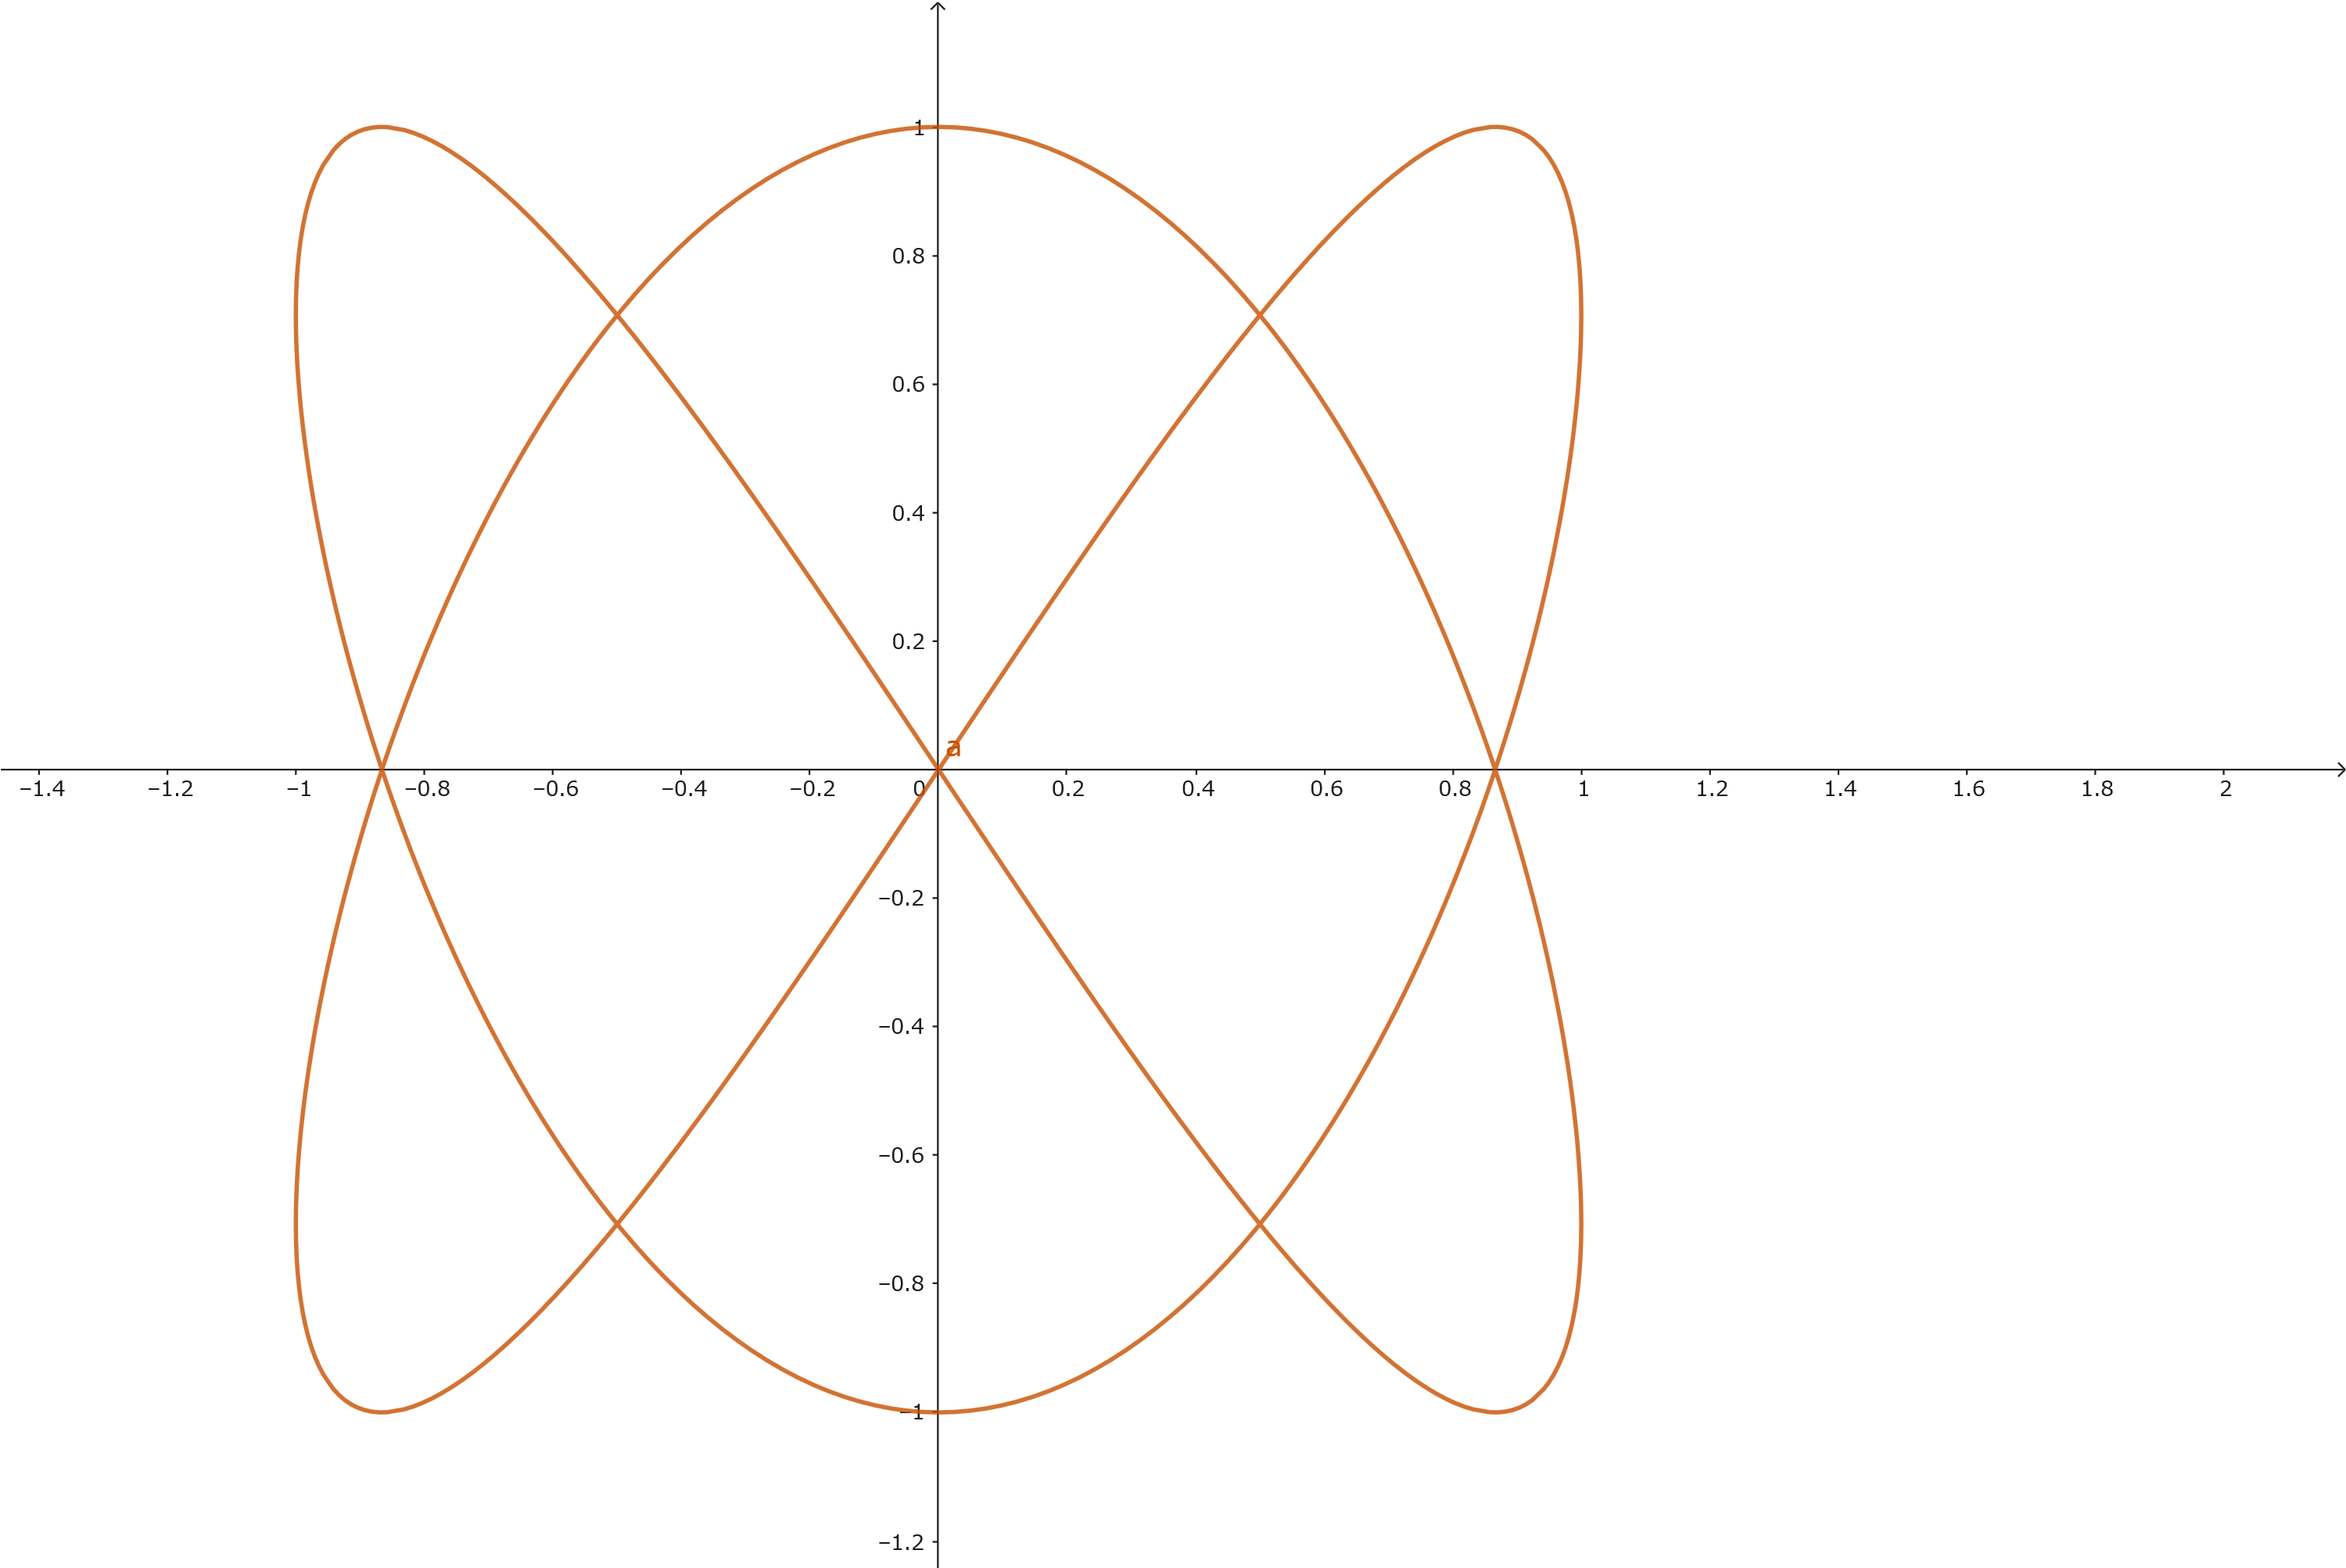
\includegraphics[width=\linewidth]{img/lissajous.png}
  \caption{リサージュ曲線($m=2,n=3$)(generated by GeoGebra)}
\end{figure}
とてもきれいですね。
電通大の校章にも使われているようです\footnote{
  https://www.uec.ac.jp/about/profile/emblem.html
}。
このように閉曲線は、自己交叉することを許可しています。
そうでないような閉曲線は名前がついています。
\begin{definition}
  平面閉曲線$(\gamma,[a,b])$が任意の$a\leq t_1<t_2\leq b$に対して$\gamma(t_1)\neq\gamma(t_2)$を満たす時、\textbf{単純閉曲線}と呼ぶ。
\end{definition}



\section{閉曲線の回転数}

リサージュ曲線のように、ぐるぐると回りまわる閉曲線には、その「\textbf{回転した回数}」が気になるところです。
絵に描いて目に見える曲線なら、それを指でなぞって数えることができますが、そうではない閉曲線にも一般に定義したいところです。

一つの考えとしては、単位接ベクトル$e_1(s)$が定義域を動くとき、これが何周したかを数えることです。
$e_1(s)$の挙動に注目すると、まず$|e_1(s)|=1$なので、$e_1$はよく考えたら円周$S^1$への写像になっています。
\begin{definition}[接線写像]
  $(\gamma,I)$を弧長パラメータ付け可能な平面曲線とし、$s=s(t)$をその弧長パラメータとする。
  このとき、写像
  \[
    e_1:s(I)\to S^1;s\mapsto e_1(s):=\frac{d\gamma(t(s))}{ds}
  \]
  を\textbf{接線写像}という。
\end{definition}

接線写像が$S^1$への写像なので、閉曲線の単位接ベクトルが$S^1$を何周したかは頑張れば定義できそうです。
それは間違いなく、僕たちが知りたい回転数になるはずです。
発想は単純ですが、これを一般論に昇華するためには、基本群で学んだ被覆空間の理論を思い出してほしいです。

\subsection{被覆空間の理論概要}
\begin{definition}[被覆空間]
  $X,\overline{X}$を位相空間とする。
  連続写像$p:\overline{X}\to X$が\textbf{被覆写像}であるとは、任意の$x\in X$に対して、$X$の開集合$U$が存在して、以下を満たす。
  \begin{itemize}
    \item $x\in U$
    \item 開集合$p^{-1}(U)$は、$p$によって$U$と同相な開集合の非交和である。
  \end{itemize}
  $p:\overline{X}\to X$が被覆写像であるとき、$\overline{X}$は$X$の\textbf{被覆空間}であるという。
\end{definition}
\begin{example}
  \[
    p:\mathbb{R}\to S^1;x\mapsto(\cos(x),\sin(x))
  \]
  は被覆写像である。
\end{example}

\begin{definition}
  $X,\overline{X},Y$を位相空間、$p:\overline{X}\to X$を被覆写像、$f:Y\to X$を連続写像とする。
  このとき、連続写像$\overline{f}:Y\to\overline{X}$であって、$p\circ\overline{f}=f$を満たすものを、連続写像$f$の$\overline{X}$への\textbf{持ち上げ}と呼ぶ。
\end{definition}
\begin{theorem}[道の持ち上げ定理]
  $X,\overline{X}$を位相空間、$p:\overline{X}\to X$を被覆写像、$I\subset\mathbb{R}$を閉区間、$f:I\to X$を連続写像とする。
  このとき、$f$の$\overline{X}$への持ち上げ$\overline{f}:I\to\overline{X}$が存在する。
\end{theorem}
\begin{example}
  $(\gamma,I)$を弧長パラメータ付け可能な平面曲線とし、$s=s(t)$をその弧長パラメータとする。
  このとき、接線写像
  \[
    e_1:s(I)\to S^1;s\mapsto e_1(s)=\frac{d\gamma(t(s))}{ds}
  \]
  は連続写像である。
  従って、接線写像の$\mathbb{R}$への持ち上げ
  \[
    \overline{e_1}:s(I)\to\mathbb{R}
  \]
  が存在する。
\end{example}

\begin{definition}[被覆変換群]
  $X,\overline{X}$を位相空間、$p:\overline{X}\to X$を被覆写像とする。
  このとき、同相写像$f:\overline{X}\to\overline{X}$であって、$p\circ f=p$を満たすものを\textbf{被覆変換}と呼ぶ。
\end{definition}
\begin{theorem}
  $X,\overline{X}$を位相空間、$p:\overline{X}\to X$を被覆写像とする。
  このとき、被覆変換全体の集合
  \[
    \operatorname{Aut}_X(\overline{X}):=\{f:\overline{X}\overset{\cong}{\longrightarrow}\overline{X}\mid p\circ f=p\}
  \]
  は、写像の合成によって群となる。
\end{theorem}
\begin{example}
  \[
    \operatorname{Aut}_{S^1}(\mathbb{R})\cong\mathbb{Z};f\mapsto \frac{f(0)}{2\pi}
  \]
  となる。実際、被覆変換は$p\circ f=f$を満たすために$f(x)=x+2\pi n$という形しか取れない。
\end{example}

\subsection{回転数}

被覆写像$p:\mathbb{R}\to S^1$に対する被覆変換群は、イメージとしては常螺旋を一段ずつ上にあげたり下げたりする操作を表わします。
一方で$\operatorname{Aut}_{S^1}(\mathbb{R})\cong\mathbb{Z}$は被覆空間に関するガロア対応によって、$S^1$の\textbf{基本群}$\pi_1(S^1)$と同型でした。
$\pi_1(S^1)\cong\mathbb{Z}$の元は、ざっくり言って「$n$回$S^1$を回る道の代表元」なのでした。
これを結びつけて行けば、被覆変換の「何段変わったか？」のイメージを閉曲線の回転数に採用できそうです。
\begin{definition}
  $(\gamma,I)$を弧長パラメータ付け可能な閉曲線とし、$s=s(t)$をその弧長パラメータとする。
  $e_1(s)$を$\gamma$の単位接ベクトルとし、これを接線写像$e_1:s(I)\to S^1$とみたときの$\mathbb{R}$への持ち上げを$\overline{e_1}:s(I)\to\mathbb{R}$とおく。
  また、$s(I)=[0,L]$であるとする(すなわち$\gamma$の長さを$L$とする)。
  \[
    w_\gamma:=\frac{\overline{e_1}(L)-\overline{e_1}(0)}{2\pi}
  \]
  を$(\gamma,I)$の\textbf{回転数}と呼ぶ。
\end{definition}
この定義でもたらされた回転数が整数であることは、被覆変換群の理論からしっかり保証されています！
\begin{figure}[htbp]
  \centering
  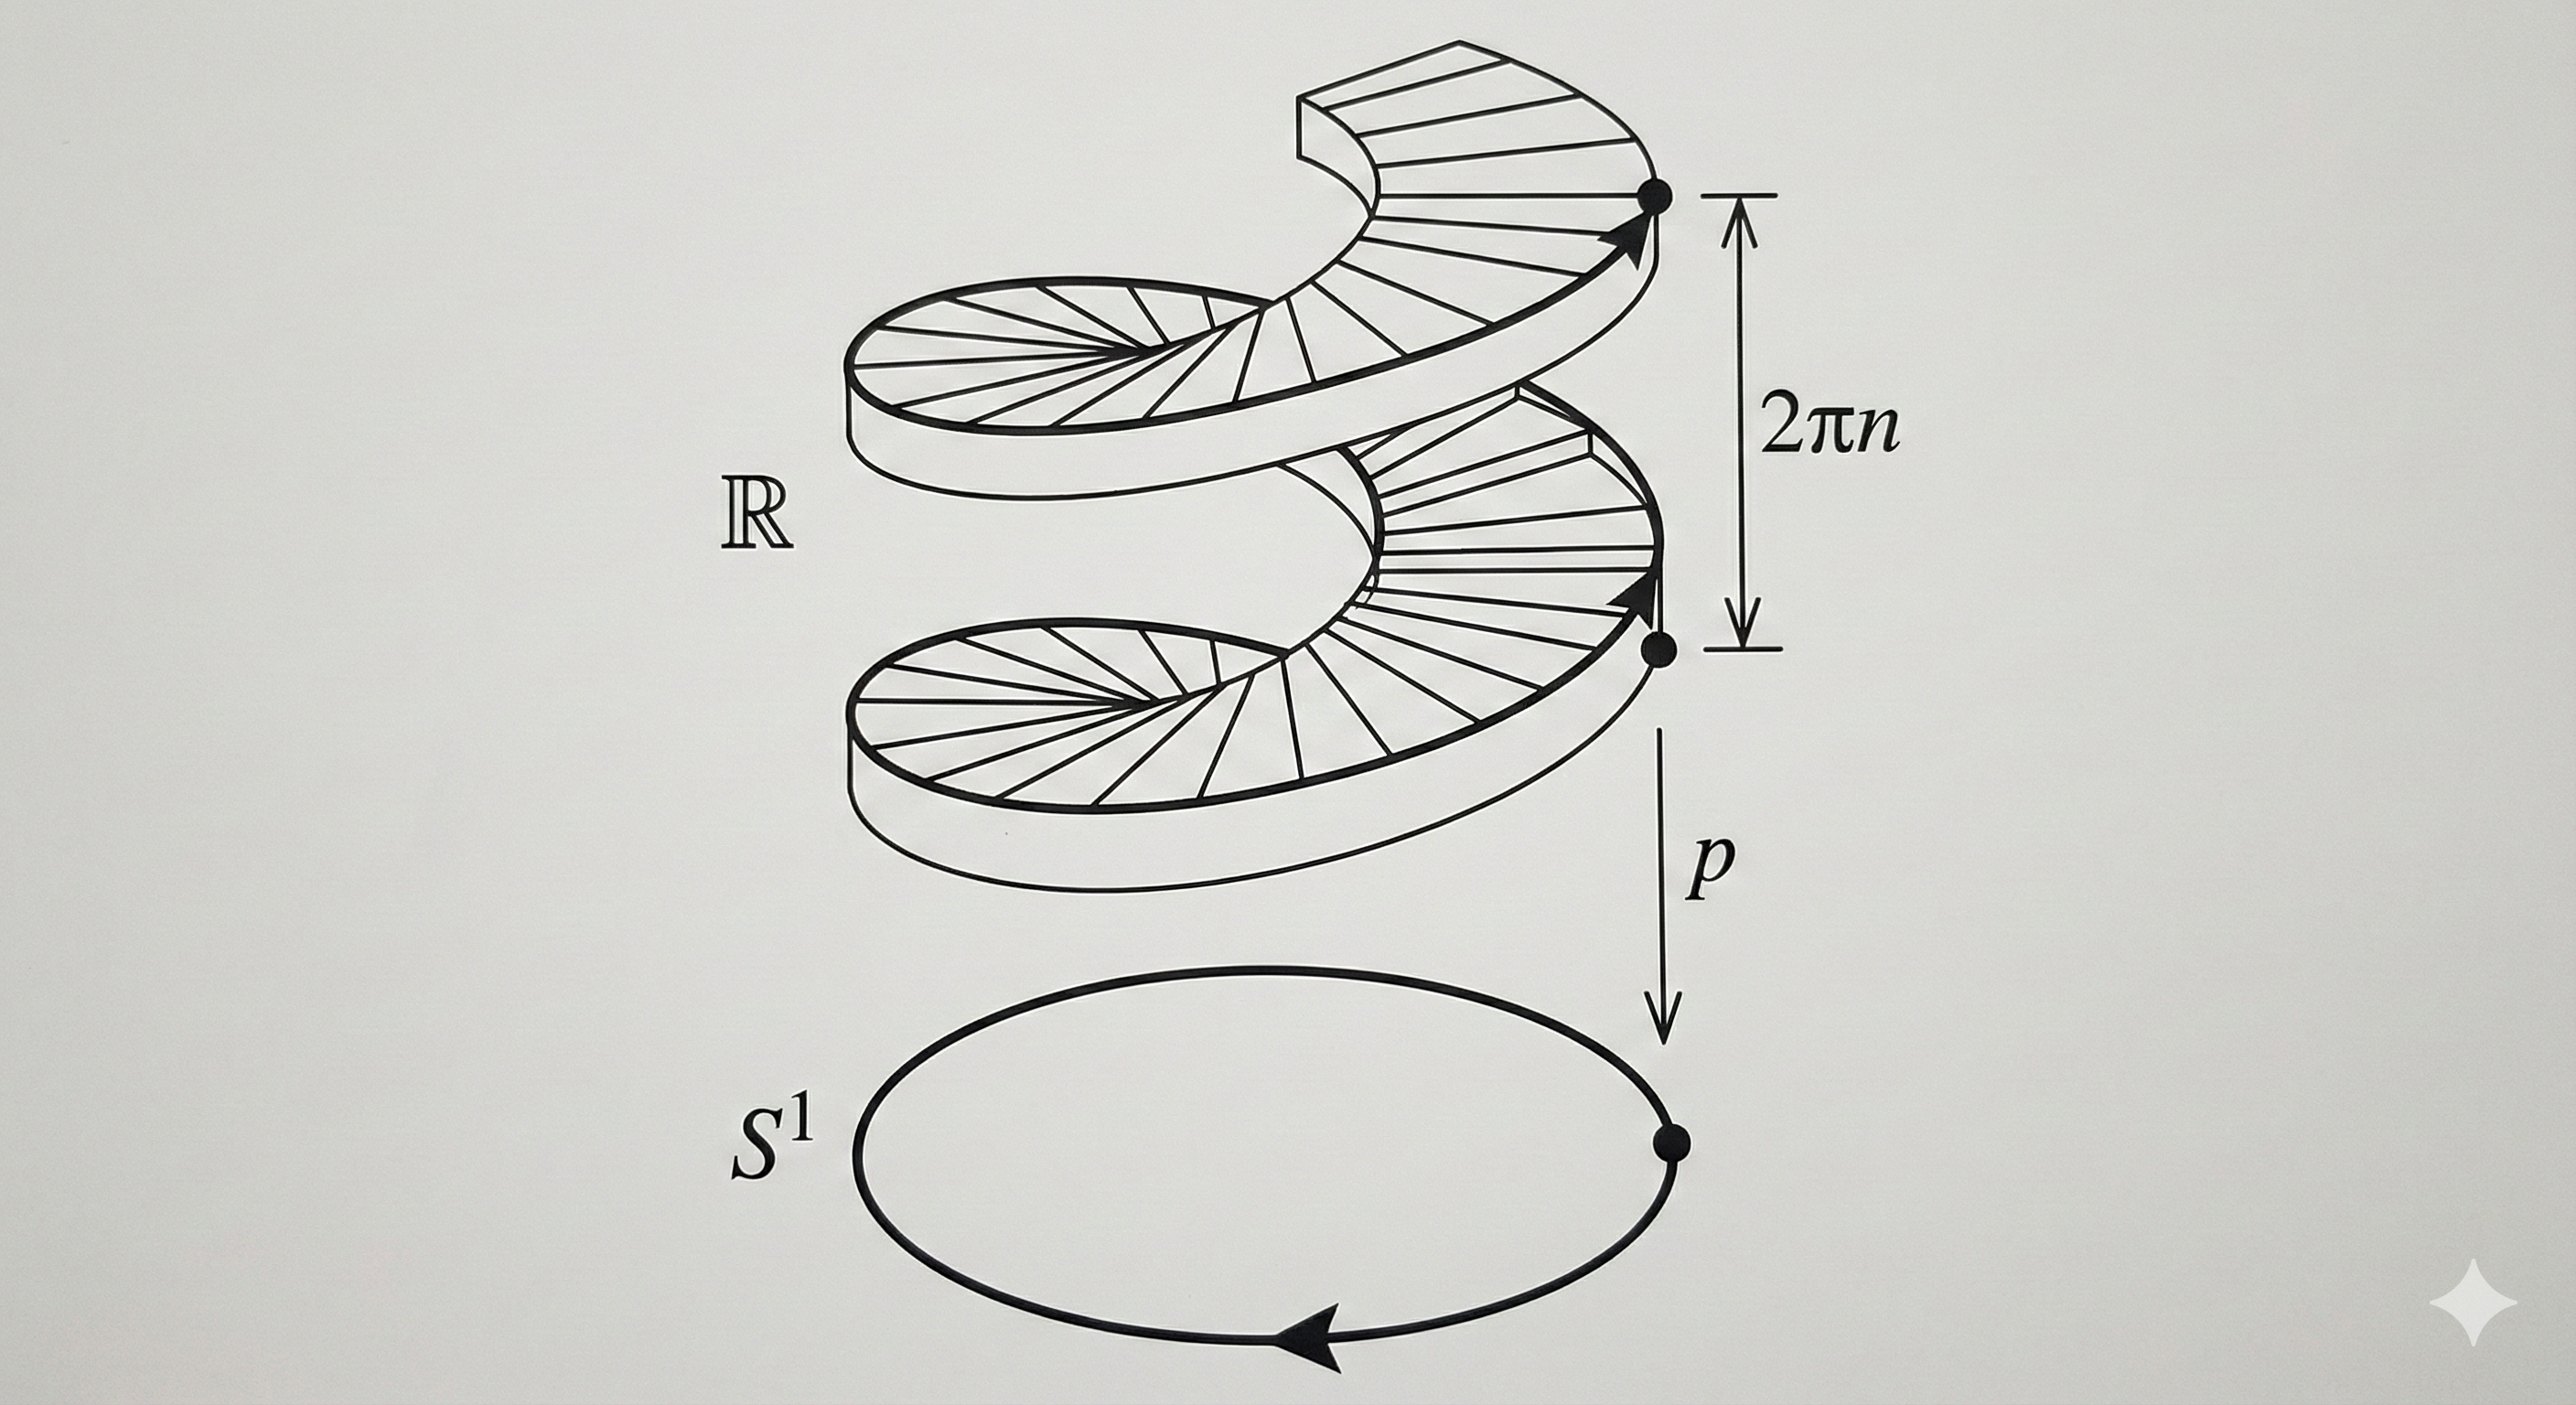
\includegraphics[width=\linewidth]{img/Gemini_Generated_Image_2isokk2isokk2iso.png}
  \caption{回転数のイメージ(generated by Gemini)}
\end{figure}

\subsection{回転数の計算例}

分かり切った計算ですが、円の回転数を求めてみましょう。
\begin{example}
  弧長パラメータ付けた円$\gamma(t(s))=(\cos(s),\sin(s))$に対して、$e_1(s)=(-\sin(s),\cos(s))$。
  接線写像とみた$e_1:[0,2\pi]\to S^1$の被覆写像$p:\mathbb{R}\to S^1;x\mapsto(\cos(x),\sin(x))$への持ち上げは、例えば
  \[
    \overline{e_1}(s)=s+\frac{\pi}{2}
  \]
  となる。
  ゆえに
  \[
    w_\gamma=\frac{\overline{e_1}(2\pi)-\overline{e_1}(0)}{2\pi}=\frac{(2\pi+\pi/2)-\pi/2}{2\pi}=1
  \]
  となる。
\end{example}
思った通りですね。

ここで残念なお知らせです。
ろくに定義から計算できる閉曲線はこれぐらいです。
なぜなら、単位接ベクトル$e_1(s)$を求めるということは、ほとんどの曲線では重労働だからです。
これは弧長パラメータの求めにくさから来ています。
例えば楕円$\gamma(t)=(a\cos(t),b\sin(t))$でさえ、その弧長は楕円積分という積分の実行が不可能な形になるのでした。
なので、もう少し議論を進めていく必要がありそうです。

\subsection{回転数と曲率の積分との関係}

まず
\[
  \overline{e_1}(L)-\overline{e_1}(0)
\]
がどんな形で表わせそうに見えますか？
例えば
\[
  \overline{e_1}(s)=\int_0^s f(\xi)d\xi
\]
という関数$f(x)$、つまり$\overline{e_1}:[0,L]\to\mathbb{R}$の原始関数があれば
\[
  \overline{e_1}(L)-\overline{e_1}(0)=\int_0^Lf(\xi)d\xi
\]
と表わせるはずです。
$f(x)$を求めるためには、$\overline{e_1}(s)=\int_0^s f(\xi)d\xi$の両辺を微分するしかないですね。
微分可能かどうかは一旦おいておいて、まずやってみましょう。
\[
  f(s)=\frac{d\overline{e_1}(s)}{ds}
\]

まだよくわからないということで、被覆写像$p:\mathbb{R}\to S^1;t\to(\cos(t),\sin(t))$を合成してみましょう。
\[
  p(f(s))=p\left(\frac{d\overline{e_1}(s)}{ds}\right)
\]
これも手が止まってしまいそうです。

もっと手前に戻りましょう。
$\overline{e_1}(s)$は$e_1(s)=p(\overline{e_1}(s))$を満たすような持ち上げでした。
この両辺を微分すれば、合成関数の微分法則から$d\overline{e_1}(s)/ds$が出てくるはずです！
\[
  \frac{de_1(s)}{ds}=\frac{dp(\overline{e_1}(s))}{ds}=\frac{d(\cos(\overline{e_1}(s)),\sin(\overline{e_1}(s)))}{ds}=\frac{d\overline{e_1}(s)}{ds}(-\sin(\overline{e_1}(s)),\cos(\overline{e_1}(s)))
\]
左辺の絶対値は空間曲線で定義した曲率$\kappa(s)$にほかなりません！
また右辺の因子のうち、
\[
  e_2(s):=(-\sin(\overline{e_1}(s)),\cos(\overline{e_1}(s)))
\]
は$e_1(s)$と直交する単位法線ベクトルになっています。
実際、長さが1になることは自明です。
また、$e_1=p\circ\overline{e_1}$であったから、実は
\[
  e_1(s)=p(\overline{e_1})=(\cos(\overline{e_1}),\sin(\overline{e_1}))
\]
と書き表せるからです。

さて、ここで一つの問題が発生します。
空間曲線の曲率は$\kappa(s)=|d^2\gamma(t(s))/ds^2|$でしたので、得られた等式
\[
  \frac{de_1(s)}{ds}=\frac{d\overline{e_1}(s)}{ds}e_2(s)
\]
から、
\[
  \kappa(s)=\left|\frac{d\overline{e_1}(s)}{ds}\right|
\]
というどこか惜しい式が出てきました。
符号が正で取れればうれしいのに…。

そこで空間曲線では、そもそもなぜ$\kappa(s)>0$となっていたことを思い出しましょう。
これは定義としては
\[
  \kappa(s):=\left|\frac{de_1(s)}{ds}\right|
\]
で平面曲線と同様なのですが、最大の目的は主法線ベクトル$e_2(s)$を定義
\[
  e_2(s):=\frac{de_1(s)/ds}{|de_1(s)/ds|}
\]
において、0除算を避けるためでした。

ところが平面曲線の場合、このような0除算を避けて法線ベクトル$e_2(s)$が先ほどの通り
\[
  e_2(s):=(-\sin(\overline{e_1}(s)),\cos(\overline{e_1}(s)))
\]
と定義されました。
であれば、そもそも曲率と呼ぶべき
\[
  \kappa(s)=\left|\frac{de_1(s)}{ds}\right|
\]
が絶対に正でなければいけないという理由もないです。
逆に自然に
\[
  \kappa_p(s)=\frac{d\overline{e_1}(s)}{ds}
\]
こそが曲率であると考えてよかろうなのです(平面(plane)の$p$を添え字につけておきました)。
であれば、次がなりたつということです！
\begin{theorem}
  $(\gamma,I)$を弧長パラメータ付け可能な閉曲線とし、$s=s(t)$をその弧長パラメータとする。
  $e_1(s)$を$\gamma$の単位接ベクトルとし、これを接線写像$e_1:s(I)\to S^1$とみたときの$\mathbb{R}$への持ち上げを$\overline{e_1}:s(I)\to\mathbb{R}$とおく。
  また、$s(I)=[0,L]$であるとする。
  このとき、次が成り立つ。
  \[
    w_\gamma=\frac1{2\pi}\int_0^L\kappa_p(s)ds
  \]
\end{theorem}
こうなるとこの関数が、以前にやった「接円の半径の逆数」としての意味をどのように持っているかが気になってくるところです。
簡単な例でいくつか確認しましょう。

\begin{example}
  半径$r>0$の円
  \[
    \gamma:[0,2\pi]\to\mathbb{R}^2;t\mapsto r(\cos(t),\sin(t))
  \]
  について考える。このとき弧長パラメータは$s(t)=rt\Leftrightarrow t(s)=s/r$である。
  ゆえに$\gamma(t(s))=r(\cos(s/r),\sin(s/r))$であり、$e_1(s)=(-\sin(s/r),\cos(s/r))$となる。
  これを$\gamma$の接線写像$e_1:[0,2\pi r]\to S^1$とみたとき、被覆空間$\mathbb{R}\to S^1;x\mapsto(\cos(x),\sin(x))$への持ち上げは、
  \[
    \overline{e_1}(s)=\frac{s}{r}+\frac{\pi}{2}
  \]
  となる。
  ゆえに平面曲線の曲率は
  \[
    \kappa_p(s)=\frac{d\overline{e_1}(s)}{ds}=\frac{1}{r}
  \]
  となり、空間曲線の曲率と一致する。

  一方で、逆回りの円
  \[
    \gamma:[0,2\pi]\to\mathbb{R}^2;t\mapsto r(\cos(-t),\sin(-t))
  \]
  について考える。このとき弧長パラメータは変わらず、$s(t)=rt\Leftrightarrow t(s)=s/r$である。
  ゆえに$\gamma(t(s))=r(\cos(-s/r),\sin(-s/r))$であり、$e_1(s)=(\sin(-s/r),-\cos(-s/r))$となる。
  これを$\gamma$の接線写像$e_1:[0,2\pi r]\to S^1$とみたとき、被覆空間$\mathbb{R}\to S^1;x\mapsto(\cos(x),\sin(x))$への持ち上げは、
  \[
    \overline{e_1}(s)=-\frac{s}{r}-\frac{\pi}{2}
  \]
  となる。
  ゆえに平面曲線の曲率は
  \[
    \kappa_p(s)=\frac{d\overline{e_1}(s)}{ds}=-\frac{1}{r}
  \]
  となる。
  これは空間曲線の曲率とは符号のみ異なる。
\end{example}
これは平面においては、曲線が時計回りか反時計回りかを、曲率によって区別することができることを意味します。
空間においては、その曲線をどこから見れば時計回りか反時計回りかが、実は区別できないです。
$z$軸の上から見れば時計回りな円でも、$z$軸の下から見れば反時計回りになります。
一方で平面曲線は、\textbf{その二次元の世界に住んでいる人々から見れば}、その曲線が時計回りか反時計回りかは一意に判別できるのです。
このような見え方の違いが、平面曲線と空間曲線で異なるのです。

遅ればせながら、平面曲線の曲率を定義しましょう。
\begin{definition}
  $(\gamma,I)$を平面曲線かつ閉曲線、$s=s(t)$をその弧長パラメータとする。
  $L$を$(\gamma,I)$の弧長とし、$e_1:[0,L]\to S^1;s\mapsto d\gamma(t(s))/ds$を接線写像とする。
  $p:\mathbb{R}\to S^1;x\mapsto(\cos(x),\sin(x))$を$S^1$の被覆写像とする。
  このとき、
  \[
    \kappa_p(s)=\frac{d\overline{e_1}(s)}{ds}
  \]
  を、曲線$(\gamma,I)$の\textbf{平面曲率}と呼ぶ。
\end{definition}

実際のところ、接線写像$e_1$の持ち上げ$\overline{e_1}$が微分可能かどうかはまだ証明していませんでした。
面倒ですが、まあ頑張って証明しましょう。
\begin{theorem}
  $(\gamma,I)$を平面曲線かつ閉曲線、$s=s(t)$をその弧長パラメータとする。
  $L$を$(\gamma,I)$の弧長とし、$e_1:[0,L]\to S^1;s\mapsto d\gamma(t(s))/ds$を接線写像とする。
  $p:\mathbb{R}\to S^1;x\mapsto(\cos(x),\sin(x))$を$S^1$の被覆写像とする。
  このとき、接線写像$e_1$の$\mathbb{R}$への持ち上げ$\overline{e_1}:[0,L]\to\mathbb{R}$は$C^1$級である。
\end{theorem}
\begin{proof}
  まず$s\in(0,L)$に対して、$p:\mathbb{R}\to S^1$は被覆写像であるから、$e_1(s)\in S^1$を含む開集合$U\subset S^1$が存在して、$p^{-1}(U)$は被覆写像$p$によって同相な開集合の非交和である。
  より小さく$U$をとって、十分小さな$\delta>0$に対して、
  \[
    U=\{(\cos(x),\sin(x))\mid |x-\overline{e_1}(s)|<\delta\}
  \]
  であるとしてよい。
  このとき$p^{-1}(U)$は、$n\in\mathbb{Z}$に対して$V_n:=\{x+2\pi n\mid |x-\overline{e_1}(s)|<\delta\}$とおけば
  \[
    p^{-1}(U)=\bigsqcup_{n\in\mathbb{Z}}V_n
  \]
  である。

  $\overline{e_1}(s)\in V_0$であるから、$V_0$に注目すると、$u\in V_0$に対して
  \[
    p|_{V_0}(u)=(\cos(u),\sin(u))
  \]
  である。
  ここで、$\gamma(t(u))=(f(u),g(u))$とおくと、$e_1(u)=d\gamma(t(u))/du$。
  また$p\circ\overline{e_1}(u)=e_1(u)$より、
  \[
    p(\overline{e_1}(u))=e_1(u)=\left(\frac{df(u)}{du},\frac{dg(u)}{du}\right)
  \]
  左辺は$(\cos(\overline{e_1}(u)),\sin(\overline{e_1}(u)))$に他ならないから、
  \[
    \begin{cases}
      \cos(\overline{e_1}(u))=\frac{df(u)}{du}\\
      \sin(\overline{e_1}(u))=\frac{dg(u)}{du}
    \end{cases}
  \]
  以下、$e_1(s)$の位置によって場合分けを行う。

  \textbf{$\cos(\overline{e_1}(s))\neq0$の場合。}
  このとき$\sin(\overline{e_1}(s))\neq\pm1$である。
  従って、必要ならばさらに$\delta>0$を小さく取り、任意の$u\in V_0$に対して
  \[
    \sin(\overline{e_1}(u))\in(0,1)
  \]
  は単調増加、あるいは単調減少であるとしてよい($\sin$のグラフを思い浮かべよ)。
  この範囲で、$\arcsin$は$C^\infty$級関数であり、
  \[
    \overline{e_1}(u)=\arcsin\left(\frac{dg(u)}{du}\right)+2k\pi
  \]
  が得られる。
  $\gamma$は$C^2$級だったから、$dg(u)/du$は$C^1$級である。
  ゆえに$\overline{e_1}(u)=\arcsin\left(\frac{dg(u)}{du}\right)+2k\pi$は$C^1$級であって、これが求めたいことであった。

  \textbf{$\cos(\overline{e_1})(s)=0$の場合。}
  このとき、必要ならばさらに$\delta>0$を小さく取り、任意の$u\in V_0$に対して
  \[
    \cos(\overline{e_1}(u))\in(0,1)
  \]
  は単調増加、あるいは単調減少であるとしてよい($\cos$のグラフを思い浮かべよ)。
  この範囲で、$\arccos$は$C^\infty$級関数であり、
  \[
    \overline{e_1}(u)=\arccos\left(\frac{df(u)}{du}\right)+2k\pi
  \]
  $\gamma$は$C^2$級だったから、$df(u)/du$は$C^1$級である。
  ゆえに$\overline{e_1}(u)=\arccos\left(\frac{df(u)}{du}\right)+2k\pi$は$C^1$級であって、これが求めたいことであった。
\end{proof}



\section{回転数と平面曲率の関係式の使用例}

平面曲線$(\gamma,I)$の平面曲率$\kappa_p:s(I)\to\mathbb{R}$の定義はとても複雑でした。
あらためて手順を説明すると、
\begin{enumerate}
  \item 弧長パラメータ$s=s(t)$を用意する
  \item 全弧長$L$を求める
  \item 単位接ベクトル$e_1$を接線写像$e_1:[0,L]\to S^1$とみる
  \item $S^1$には被覆空間$p:\mathbb{R}\to S^1;t\mapsto(\cos(t),\sin(t))$があった
  \item 接線写像$e_1$の$\mathbb{R}$への持ち上げ$\overline{e_1}:[0,L]\to\mathbb{R}$は$C^1$級
  \item このとき、平面曲率は
  \[
    \kappa_p:[0,L]\to\mathbb{R};s\mapsto\frac{d\overline{e_1}(s)}{ds}
  \]
  で定義される。
\end{enumerate}
このとき、$\gamma$の回転数$w_\gamma$は
\[
  w_\gamma=\frac1{2\pi}\int_0^L\kappa_p(s)ds
\]
で求められるのでした。
$\kappa_p(s)$という局所的に定義したものを積分が$2\pi$の整数倍になるのが驚きですね。
しかもその整数というのが、位相的には見た目で計算できる回転数になるのは凄いと思います。
例えば楕円
\[
  \gamma(t)=(a\cos(t),b\sin(t))
\]
で上の手順で$\int\kappa_p(s)ds$を求めようとするとめちゃくちゃ大変ですが、もう$S^1$と同相なので
\[
  \int_0^L\kappa_p(s)ds=2\pi w_{\text{楕円}}=2\pi
\]
と求まります。

リサージュ曲線の曲率の場合、逆に目で追うのが大変ですが、$\kappa_p$を積分することで0になることがわかります。
実は(例\ref{example:Lissajous_curve}の)リサージュ曲線の回転数はすべて0です。
例えば$(m,n)=(1,2)$のリサージュ曲線はこんな形になります。
\begin{figure}[htbp]
  \centering
  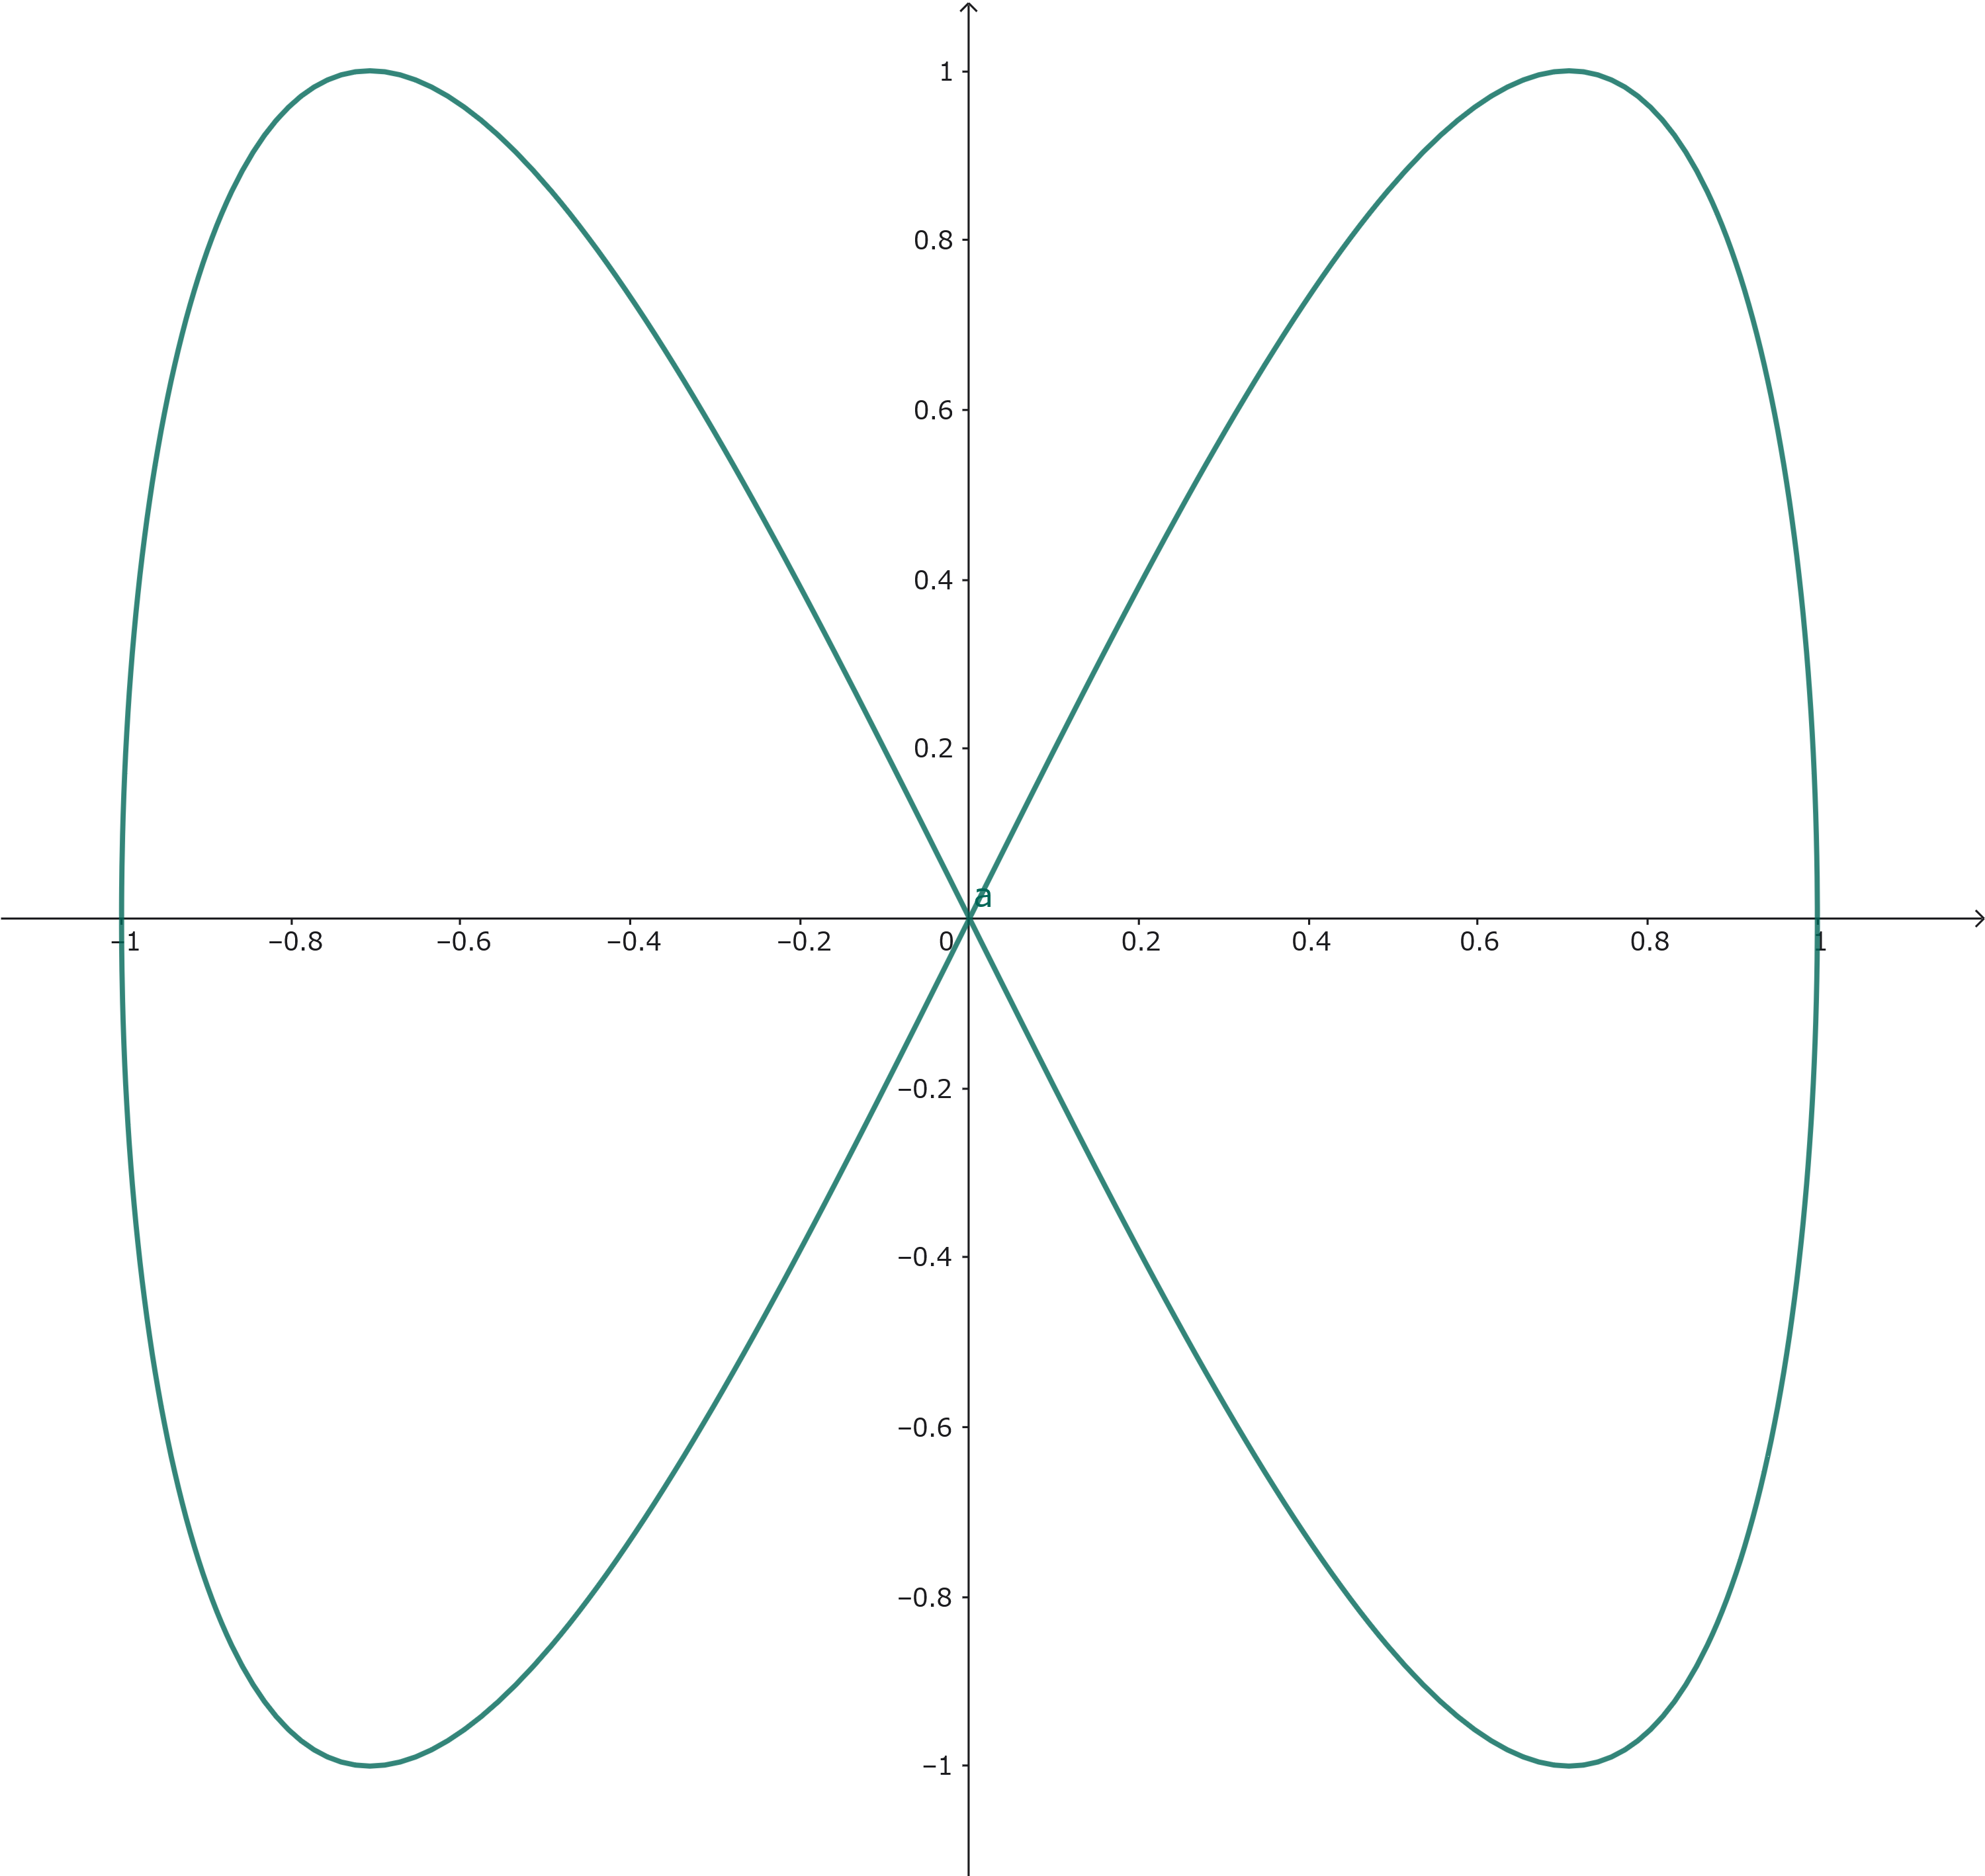
\includegraphics[scale=2.0]{img/Lissajous_curve_1_2.png}
  \caption{($m=1,n=2$)(generated by GeoGebra)}
\end{figure}
マリオカートか何かで、このような形のサーキットがあったと思います。
ともかくこのサーキットで原点から車を走らせると、まず第一象限から第四象限にいる間は、右方向にハンドルを曲げなければいけません。
第四象限を抜けて、第二象限に突入すると、ハンドルを左方向に曲げ無ければいけません。
そして一周して戻ってくる。
合計の回転数は左右が打ち消しあって0というわけです。

一般の場合に示してみましょう。
\begin{theorem}
  $m, n \in \mathbb{Z} \setminus \{0\}$ を互いに素な整数とし、その和 $m+n$ は奇数であるとする（すなわち偶奇が異なる）。
  このとき、閉曲線
  \[
    \gamma: [0, 2\pi] \to \mathbb{R}^2, \quad \gamma(t) = (\sin(mt), \sin(nt))
  \]
  の回転数は $0$ である。
\end{theorem}
\begin{proof}
  まずは平面曲率を求めるために、弧長パラメータを定義しておくと、
  \[
    s(t)=\int_0^t \sqrt{m^2\cos^2(mt)+n^2\cos^2(nt)} \, dt
  \]
  となる。
  すると
  \[
    e_1(s):=\frac{d\gamma(t(s))}{ds}=\frac{dt}{ds}\frac{d\gamma(t)}{dt}=\frac{(m\cos(mt),n\cos(nt))}{\sqrt{m^2\cos^2(mt)+n^2\cos^2(nt)}}
  \]
  となる。
  一旦、このまま$\mathbb{R}$に持ち上げて
  \[
    \overline{e_1}:[0,L]\to\mathbb{R}
  \]
  を作ります。
  このとき、単位接ベクトルと単位法ベクトルは
  \begin{align*}
    e_1(s)&=(\cos(\overline{e_1}(s)),\sin(\overline{e_1}(s)))\\
    e_2(s)&=(-\sin(\overline{e_1}(s)),\cos(\overline{e_1}(s)))
  \end{align*}
  であるから、$de_1(s)/ds$から$d\overline{e_1}(s)/ds=:\kappa_p(s)$が出てくる。
  \[
    \kappa_p(s)=\frac{de_1(s)}{ds}\cdot e_2(s)
  \]
  さらに計算を進めると、$e_1(s)$から結果的に$e_2(s)$の各成分を知ることができる。
  \begin{align*}
    e_1(s)&=(\cos(\overline{e_1}(s)),\sin(\overline{e_1}(s)))=p(\overline{e_1}(s))=\frac{(m\cos(mt),n\cos(nt))}{\sqrt{m^2\cos^2(mt)+n^2\cos^2(nt)}}\\
    e_2(s)&=(-\sin(\overline{e_1}(s)),\cos(\overline{e_1}(s)))=\frac{(-n\cos(nt),m\cos(mt))}{\sqrt{m^2\cos^2(mt)+n^2\cos^2(nt)}}
  \end{align*}
  ここで $m, n$ は互いに素かつ和が奇数であるため、$\cos(mt)$ と $\cos(nt)$ が同時に $0$ になることはなく、$d\gamma(t)/dt \neq 0$ が保証されることに注意する。
  これによって$\kappa_p$が以下のように求まる。
  \begin{align*}
    \frac{de_1(s)}{ds}=\frac{mn(n\sin(nt)\cos(mt)-m\sin(mt)\cos(nt))}{(m^2\cos^2(mt)+n^2\cos^2(nt))^{3/2}}(n\cos(nt),-m\cos(mt))
  \end{align*}
  ゆえに
  \[
    \kappa_p=\frac{de_1(s)}{ds}\cdot e_2(s)=\frac{mn(n\sin(nt)\cos(mt)-m\sin(mt)\cos(nt))}{m^2\cos^2(mt)+n^2\cos^2(nt)}
  \]
  となる。ゆえに$L$をリサージュ曲線の全弧長として
  \begin{align*}
    \int_0^L\kappa_p(s)ds=&\int_0^{L}\frac{mn(n\sin(nt)\cos(mt)-m\sin(mt)\cos(nt))}{m^2\cos^2(mt)+n^2\cos^2(nt)}ds\\
    =&\int_0^{2\pi}\frac{mn(n\sin(nt)\cos(mt)-m\sin(mt)\cos(nt))}{m^2\cos^2(mt)+n^2\cos^2(nt)}\frac{ds}{dt}dt\\
    =&\int_0^{2\pi}\frac{mn(n\sin(nt)\cos(mt)-m\sin(mt)\cos(nt))}{\sqrt{m^2\cos^2(mt)+n^2\cos^2(nt)}}dt
  \end{align*}
  を計算しなければならない。
  ところが
  \begin{align*}
    \cos(n(t+\pi))=(-1)^n\cos(nt)&,\quad \sin(n(t+\pi))=(-1)^n\sin(nt)\\
    \cos(m(t+\pi))=(-1)^m\cos(mt)&,\quad \sin(m(t+\pi))=(-1)^m\sin(mt)
  \end{align*}
  ゆえ、一旦
  \[
    f(t):=\frac{mn(n\sin(nt)\cos(mt)-m\sin(mt)\cos(nt))}{\sqrt{m^2\cos^2(mt)+n^2\cos^2(nt)}}
  \]
  とおくと、
  \begin{align*}
    f(t+\pi)&=\frac{mn(n\sin(n(t+\pi))\cos(m(t+\pi))-m\sin(m(t+\pi))\cos(n(t+\pi)))}{\sqrt{m^2\cos^2(m(t+\pi))+n^2\cos^2(n(t+\pi))}}\\
    &=\frac{mn(n(-1)^{n+m}\sin(nt)\cos(mt)-m(-1)^{n+m}\sin(mt)\cos(nt))}{\sqrt{m^2\cos^2(mt)+n^2\cos^2(nt)}}\\
    &=(-1)^{n+m}f(t)\\
    &=-f(t)
  \end{align*}
  となる。最後の等式で、$n+m$が奇数だったことを使った。
  以上より
  \begin{align*}
    \int_0^L\kappa_p(s)ds=&\int_0^{2\pi}f(t)dt=\int_0^\pi f(t)dt+\int_\pi^{2\pi}f(t)dt\\
    =&\int_0^\pi f(t)dt+\int_0^\pi f(t+\pi)dt\\
    =&\int_0^\pi f(t)dt-\int_0^\pi f(t)dt\\
    =&0
  \end{align*}

  ゆえにリサージュ曲線の回転数$w$は、
  \begin{align*}
    w=\frac1{2\pi}\int_0^L\kappa_p(s)ds=0
  \end{align*}
\end{proof}

\vspace{1em}

% TikZによる図解
\begin{figure}[h]
  \centering
  \begin{tikzpicture}[scale=2, >=latex]
    % 設定: m=1(奇), n=2(偶) -> y軸対称のケース
    
    % --- 左図: 接平面(velocity space)での対称性 ---
    \begin{scope}
      \draw[->, thick] (-1.5,0) -- (1.5,0) node[right] {$x'$};
      \draw[->, thick] (0,-1.5) -- (0,1.5) node[above] {$y'$};
      \draw[thick, gray!50] (0,0) circle (1); % 単位円 S^1
      
      % ベクトル v = psi(t)
      \draw[->, ultra thick, blue] (0,0) -- (60:1) node[midway, fill=white, inner sep=1pt] {$t$};
      \fill[blue] (60:1) circle (1pt);
      
      % ベクトル R(v) = psi(t+pi) (y軸対称)
      \draw[->, ultra thick, red] (0,0) -- (120:1) node[midway, fill=white, inner sep=1pt] {$t+\pi$};
      \fill[red] (120:1) circle (1pt);
      
      % 対称性の補助線
      \draw[dashed, thin] (60:1) -- (120:1);
      \node[below] at (0,-1.1) {\small $m$:奇, $n$:偶 $\implies R_y$ (左右反転)};
    \end{scope}

    % --- 右図: 概念図 ---
    \begin{scope}[xshift=4cm]
       \node[align=left, text width=4cm] at (0,0) {
         \textbf{直観的解釈:}\\
         時間が $\pi$ 進むと、接線ベクトルは鏡に映った位置へ移動する。\\
         \vspace{0.5em}
         もし回転数が $k$ ならば、\\
         前半: $k/2$ 回転\\
         後半: $-k/2$ 回転 (鏡像)\\
         \vspace{0.5em}
         合計 $k$ になるためには\\
         $k = -k \iff k=0$\\
         でなければならない。
       };
    \end{scope}
  \end{tikzpicture}
  \caption{接線写像の対称性（$m$が奇数、$n$が偶数の場合）}
\end{figure}
\begin{figure}[htbp]
  \centering
  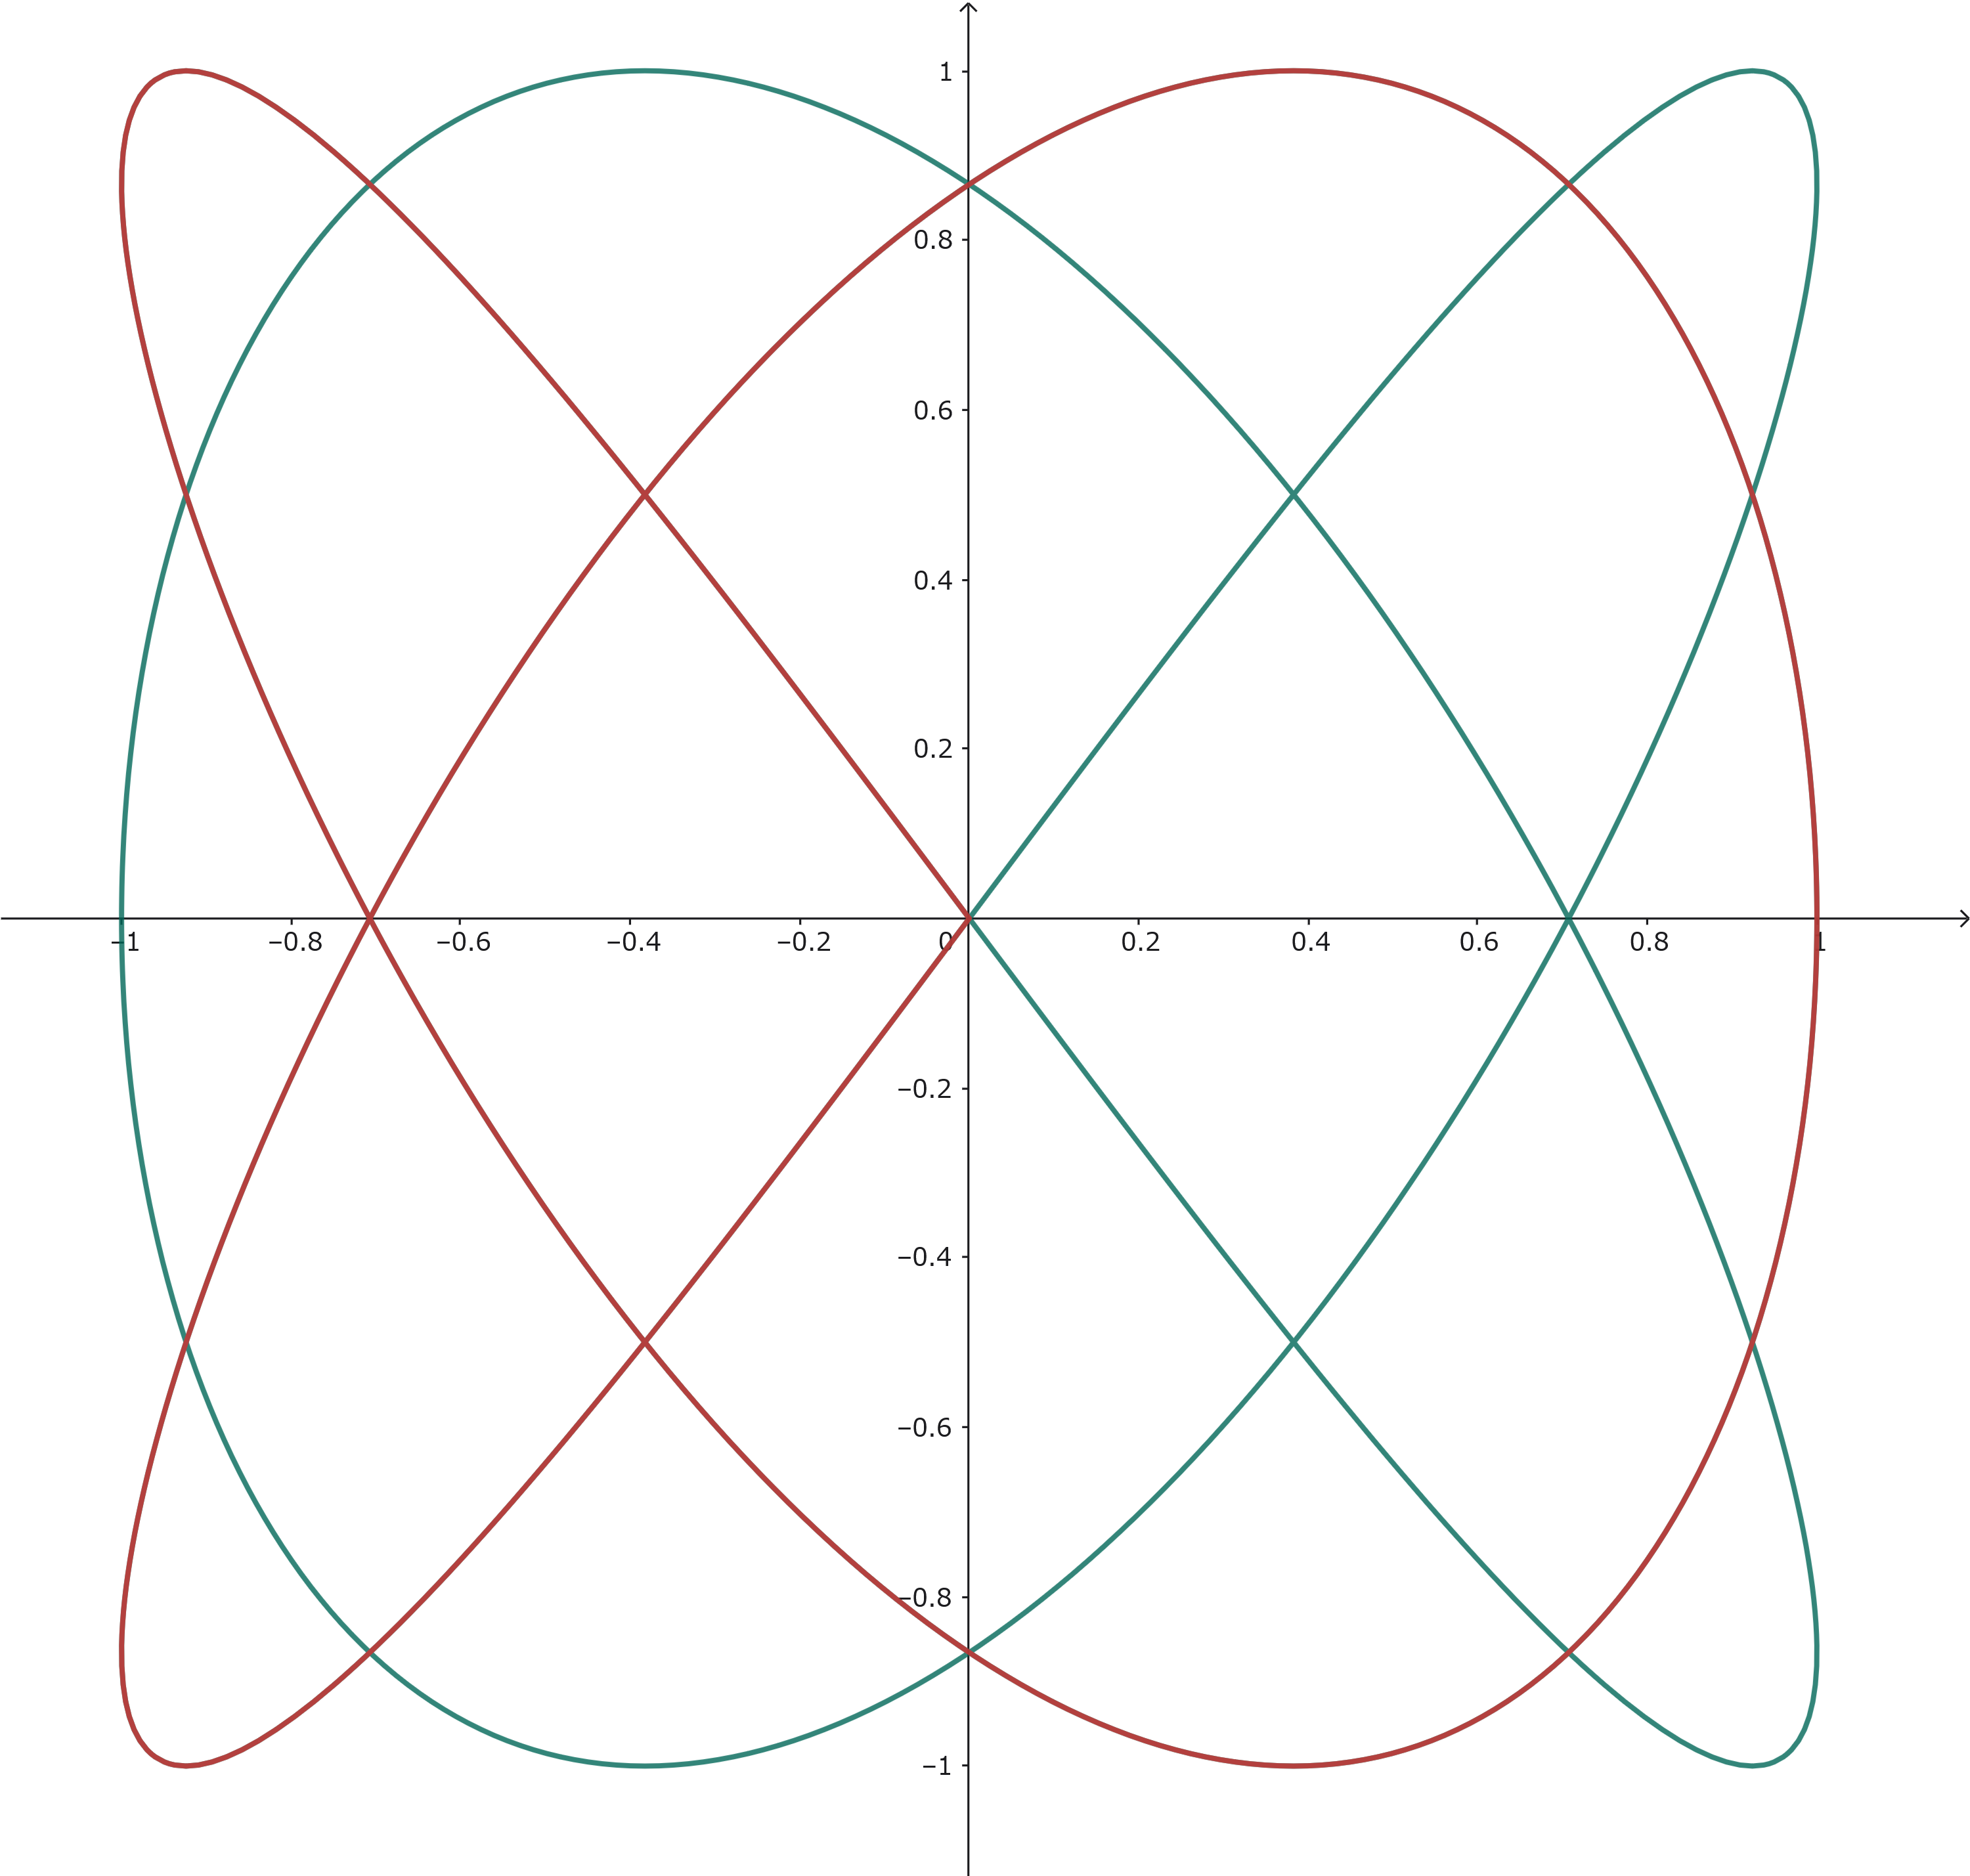
\includegraphics[scale=2.0]{img/Lissajous_curve_3_4.png}
  \caption{$m=3,n=4$。緑が$t=0\sim\pi$、赤が$t=\pi\sim2\pi$。(generated by GeoGebra)}
\end{figure}
  \part{曲面}
  \chapter{フレネ・セレの公式の応用1}

\section{曲率と捩率が定数となる曲線}

\section{例題：$\kappa>0$、$\tau=0$ならば円の一部}

\section{例題：$\kappa>0$、$\tau\neq0$が定数ならば常螺旋}

  \chapter{曲線論の基本定理}

\section{主張}

\section{証明}

  \chapter{平面曲線の理論}

\section{主張}

\section{証明}

  \chapter{物理学との関連}

\section{質点の運動とフレネ標構：加速度の接線方向と法線成分}

\section{電磁場中の荷電粒子の運動(ローレンツ力)}

  \chapter{工学分野への応用}

\section{土木・建築：高速道路や鉄道の緩和曲線（クロソイド曲線）。曲率が弧長に比例し、ハンドル操作を滑らかにする。}

\section{機械工学：カムや歯車の滑らかな形状設計、ロボットアームの軌道計画。}

\section{コンピュータグラフィックス (CG)：ベジェ曲線やスプライン曲線による自由曲線の設計と、その曲率の制御。}

  \part{Appendix}
  \chapter{補足}

\section{線形代数}

ここではガロア理論で学んだ程度の線形代数をスタートラインに、曲線論や曲面論で使う程度の線形代数を用意します。

\subsection{前提知識}

以下はガロア理論のときに証明した内容ですので、証明を割愛して述べるにとどめます。
\begin{definition}[体]
  $(K,+,\cdot,0,1)$が体であるとは、次を満たす時を言う。
  \begin{itemize}
    \item \textbf{演算の存在}: 写像$+:K\times K\to K$と$\cdot:K\times K\to K$が定められている。
      $+$を$K$の加法、$\cdot$を$K$の乗法と呼ぶ。
    \item \textbf{加法に関して可換群をなす}
    \begin{itemize}
      \item \textbf{結合法則} $a+(b+c)=(a+b)+c$ (${}^\forall a,b,c\in K$)
      \item \textbf{単位元の存在} $a+0=0+a=a$ (${}^\forall a\in K$)
      \item \textbf{逆元の存在} ${}^\forall a\in K$に対して、${}^\exists -a\in K$ s.t. $a+(-a)=(-a)+a=0$
      \item \textbf{可換性} $a+b=b+a$ (${}^\forall a,b\in K$)
    \end{itemize}
    \item \textbf{乗法に関して可換モノイドをなす}
    \begin{itemize}
      \item \textbf{結合法則} $a(bc)=(ab)c$ (${}^\forall a,b,c\in K$)
      \item \textbf{単位元の存在} $a\cdot1=1\cdot a=a$ (${}^\forall a\in K$)
      \item \textbf{可換性} $ab=ba$ (${}^\forall a,b\in K$)
    \end{itemize}
    \item \textbf{分配法則を満たす} $a(b+c)=ab+ac$ (${}^\forall a,b,c\in K$)
    \item \textbf{0以外の元は乗法に関して逆元をもつ} ${}^\forall a\in K\setminus\{0\}$に対して、${}^\exists a^{-1}\in K$ s.t. $aa^{-1}=a^{-1}a=1$
  \end{itemize}
\end{definition}
\begin{definition}[ベクトル空間]
  可換群$V$が体$K$上のベクトル空間である(以下$K$ベクトル空間)とは、スカラー倍
  \[
    K\times V\to V
  \]
  が定義されていて、次を満たす時を言う。
  \begin{itemize}
    \item \textbf{結合法則} $(ab)v=a(bv)$ (${}^\forall a,b\in K, v\in V$)
    \item \textbf{スカラーに関する分配法則} $(a+b)v=av+bv$ (${}^\forall a,b\in K, v\in V$)
    \item \textbf{ベクトルに関する分配法則} $a(v+w)=av+aw$ (${}^\forall a\in K, v,w\in V$)
    \item $1\cdot v=v$ ($\forall v\in V$)
  \end{itemize}
\end{definition}
\begin{definition}[部分空間]
  $V$を$K$ベクトル空間、$W\subset V$とする。
  $W$が$V$の部分空間であるとは、次を満たす時を言う。
  \begin{itemize}
    \item \textbf{零元の存在} $0\in W$
    \item \textbf{加法に関して閉じている} $v,w\in W\implies v+w\in W$
    \item \textbf{スカラー倍に関して閉じている} $a\in K, v\in W\implies av\in W$
  \end{itemize}
\end{definition}
\begin{definition}[商空間]
  $V$を$K$ベクトル空間、$W\subset V$を部分空間とする。
  $W$の剰余類全体の集合
  \[
    V/W:=\{v+W\mid v\in V\}
  \]
  を$V$の$W$による商空間という。
\end{definition}
\begin{definition}[一次独立]
  $K$ベクトル空間の空でない部分集合$B\subset K$が一次独立であるとは、次を満たす時を言う。
  \begin{align*}
    {}^\forall e_1,\dots,e_n\in B: \text{有限部分集合,} {}^\forall a_1,\dots,a_n\in K, \left[\sum_{i=1}^na_ie_i=0\implies a_1=\cdots=a_n=0\right]
  \end{align*}
\end{definition}
\begin{definition}[生成系]
  $K$ベクトル空間の空でない部分集合$B\subset K$が$V$の生成系であるとは、次を満たす時を言う。
  \begin{align*}
    {}^\forall v\in V, {}^\exists e_1,\dots,e_n\in B: \text{有限部分集合}, {}^\exists a_1,\dots,a_n\in K s.t. \left[v=\sum_{i=1}^na_ie_i\right]
  \end{align*}
\end{definition}
\begin{definition}[基底]
  $K$ベクトル空間$V$の空でない部分集合$B\subset K$が$V$の基底であるとは、$B$が一次独立かつ生成系であるときをいう。
  有限個の基底を選択できるとき、ベクトル空間$V$は有限次元であるといい、その基底の個数を$\dim_K(V)$で表す。
  有限次元ではないベクトル空間を無限次元ベクトル空間といい、$\dim_K(V)=+\infty$と書き表す。
  $V$が有限次元で、$B=\{e_1,\dots,e_n\}$のとき、$e_1,\dots,e_n$が基底であることを
  \[
    V=\left<e_1,\dots,e_n\right>_K
  \]
  で表す。
\end{definition}
\begin{theorem}[基底の存在と濃度の一意性]
  任意の$K$ベクトル空間は基底をもち、その濃度は基底の取り方によらず一定である。
\end{theorem}
\begin{definition}[線形写像]
  $V,W$を$K$ベクトル空間とする。
  群準同型写像$f:V\to W$が$K$線形写像であるとは、
  \[
    f(av)=af(v),\quad{}^\forall a\in K, v\in V
  \]
  を満たす時を言う。
  $f^{-1}:W\to V$が存在するとき、$f$は同型写像であるといい、$V$と$W$は互いに同型であるという。
\end{definition}
\begin{theorem}[線形写像の準同型定理]
  $V,W$を$K$ベクトル空間、$f:V\to W$を$K$線形写像とする。
  このとき、次の写像は同型写像である。
  \[
    V/{\rm Ker}(f)\to{\rm Im}(f);v+{\rm Ker}(f)\mapsto f(v)
  \]
\end{theorem}
\begin{theorem}
  $V,W$を$K$ベクトル空間、$f:V\to W$を$K$線形写像とする。
  このとき、$f$が同型写像であることと、$f$が単射かつ、$V$と$W$の次元がそれぞれ等しいことは同値である。
  特に、$V$と$W$が互いに同型であることと、それぞれの基底の濃度が等しいことは同値である。
\end{theorem}
\begin{theorem}[線形写像の行列表示]
  $V,W$を有限次元$K$ベクトル空間、$f:V\to W$を線形写像、
  \begin{align*}
    B_V&=\{e_1,\dots,e_m\}\\
    B_W&=\{e'_1,\dots,e'_n\}
  \end{align*}
  をそれぞれ$V,W$の基底とする。
  このとき、
  \[
    f(e_i)=\sum_{j=1}^ma_{ij}e'_j
  \]
  とおくことができる。このとき線形写像$f$は、行列表示
  \begin{align*}
    f(e_1,e_2,\dots,e_m)=(e'_1,e'_2,\dots,e'_n)\begin{pmatrix}
      a_{11} & a_{12} & \cdots & a_{1m}\\
      a_{21} & a_{22} & \cdots & a_{2m}\\
      \vdots & \vdots & \ddots & \vdots\\
      a_{n1} & a_{n2} & \cdots & a_{nm}\\
    \end{pmatrix}
  \end{align*}
  で特徴づけられる。
  行列
  \[
    \begin{pmatrix}
      a_{11} & a_{12} & \cdots & a_{1m}\\
      a_{21} & a_{22} & \cdots & a_{2m}\\
      \vdots & \vdots & \ddots & \vdots\\
      a_{n1} & a_{n2} & \cdots & a_{nm}\\
    \end{pmatrix}
  \]
  を、線形写像$f$の表現行列という。
\end{theorem}
\begin{theorem}
  $V_1,V_2,V_3$を$K$ベクトル空間、$f_1:V_1\to V_2$および$f_2:V_2\to V_3$を$K$線形写像とする。
  このとき$f_2\circ f_1:V_1\to V_3$はまた$K$線形写像である。
  $\dim_K(V_1)=l<+\infty$、$\dim_K(V_2)=m<+\infty$、$\dim_K(V_3)=n<+\infty$のとき、それぞれのある基底をとり、$f_1$と$f_2$の表現行列をそれぞれ
  \[
    \begin{pmatrix}
      a_{11} & a_{12} & \cdots & a_{1l}\\
      a_{21} & a_{22} & \cdots & a_{2l}\\
      \vdots & \vdots & \ddots & \vdots\\
      a_{m1} & a_{m2} & \cdots & a_{ml}\\
    \end{pmatrix},\quad
    \begin{pmatrix}
      b_{11} & b_{12} & \cdots & b_{1m}\\
      b_{21} & b_{22} & \cdots & b_{2m}\\
      \vdots & \vdots & \ddots & \vdots\\
      b_{n1} & b_{n2} & \cdots & b_{nm}\\
    \end{pmatrix}
  \]
  とする。このとき、$f_2\circ f_1$の表現行列は、行列の積
  \[
    \begin{pmatrix}
      b_{11} & b_{12} & \cdots & b_{1m}\\
      b_{21} & b_{22} & \cdots & b_{2m}\\
      \vdots & \vdots & \ddots & \vdots\\
      b_{n1} & b_{n2} & \cdots & b_{nm}\\
    \end{pmatrix}
    \begin{pmatrix}
      a_{11} & a_{12} & \cdots & a_{1l}\\
      a_{21} & a_{22} & \cdots & a_{2l}\\
      \vdots & \vdots & \ddots & \vdots\\
      a_{m1} & a_{m2} & \cdots & a_{ml}\\
    \end{pmatrix}
    =
    \begin{pmatrix}
      \sum_kb_{1k}a_{k1} & \sum_kb_{1k}a_{k2} & \cdots & \sum_kb_{1k}a_{kl}\\
      \sum_kb_{2k}a_{k1} & \sum_kb_{2k}a_{k2} & \cdots & \sum_kb_{2k}a_{kl}\\
      \vdots & \vdots & \ddots & \vdots\\
      \sum_kb_{nk}a_{k1} & \sum_kb_{nk}a_{k2} & \cdots & \sum_kb_{nk}a_{kl}\\
    \end{pmatrix}
  \]
  で表現される。
\end{theorem}

\subsection{連立一次方程式と行列式}

行列は連立一次方程式を解くのに便利です。
$V,W$を$K$有限次元ベクトル空間とし、$f:V\to W$を線形写像とします。
今回は
\[
  f(x)=c
\]
という方程式を考えましょう。
$\dim_K(V)=m$、$\dim_K(W)=n$、$V=\left<e_1,\dots,e_m\right>_K$、$W=\left<e'_1,\dots,e'_m\right>_K$とすると、$f$の表現行列を
\[
  \begin{pmatrix}
    a_{11} & a_{12} & \cdots & a_{1m}\\
    a_{21} & a_{22} & \cdots & a_{2m}\\
    \vdots & \vdots & \ddots & \vdots\\
    a_{n1} & a_{n2} & \cdots & a_{nm}\\
  \end{pmatrix}
\]
とおくことができます。
また、
\[
  x=\sum_{i=1}^mx_ie_i,\quad c=\sum_{j=1}^nc_je'_j
\]
とすると、方程式$f(x)=c$は次のように書き直すことができます。
\begin{align*}
  f\left(\sum_{i=1}^mx_ie_i\right)=c
  \iff&f(e_1,\dots,e_m)\begin{pmatrix}
    x_1\\\vdots\\x_m
  \end{pmatrix}=c\\
  \iff&(e'_1,\dots,e'_n)\begin{pmatrix}
    a_{11} & a_{12} & \cdots & a_{1m}\\
    a_{21} & a_{22} & \cdots & a_{2m}\\
    \vdots & \vdots & \ddots & \vdots\\
    a_{n1} & a_{n2} & \cdots & a_{nm}\\
  \end{pmatrix}
  \begin{pmatrix}
    x_1\\x_2\\\vdots\\x_m
  \end{pmatrix}=c\\
  \iff&\begin{pmatrix}
    a_{11} & a_{12} & \cdots & a_{1m}\\
    a_{21} & a_{22} & \cdots & a_{2m}\\
    \vdots & \vdots & \ddots & \vdots\\
    a_{n1} & a_{n2} & \cdots & a_{nm}\\
  \end{pmatrix}
  \begin{pmatrix}
    x_1\\x_2\\\vdots\\x_m
  \end{pmatrix}=
  \begin{pmatrix}
    c_1\\c_2\\\vdots\\c_n
  \end{pmatrix}
\end{align*}
ゆえに方程式$f(x)=c$は
\begin{align*}
  \begin{cases}
    a_{11}x_1+a_{12}x_2+\cdots+a_{1m}x_m=c_1\\
    a_{21}x_1+a_{22}x_2+\cdots+a_{2m}x_m=c_2\\
    \quad\vdots\\
    a_{n1}x_1+a_{n2}x_2+\cdots+a_{nm}x_m=c_n\\
  \end{cases}
\end{align*}
と同値です。
みごとに中学生以来慣れ親しんだ連立一次方程式になりました。

連立一次方程式を解くための方法の一つに、\textbf{加減法}があります。
例えば$a_{11}\neq0$のとき、第二式から第一式$\times a_{11}^{-1}a_{21}$を引いて
\[
  (a_{22}-a_{11}^{-1}a_{21}a_{12})x_2+(a_{23}-a_{11}^{-1}a_{21}a_{13})x_3+\cdots+(a_{2m}-a_{11}^{-1}a_{21}a_{1m})x_m=c_2-a_{11}^{-1}a_{21}c_1
\]
という$x_1$が消えた方程式が現れます。
第三式以降も同様で、最終的に$x_1$が残るのは第一式のみになります。
そうすると第二式以降で$x_2$の係数が生き残っているやつを選んで、$x_2$が残っている方程式が一つだけになるようにできます。
これを繰り返して$x_i$を確定していくのです。
これを一般化すると、次のような手続きになります。
\begin{definition}
  $n$を整数、$1\leq i<j\leq n$とする。
  $\alpha\delta-\beta\gamma\neq0$とする。
  このとき$n$次正方行列\footnote{行数と列数が等しい行列}
  \[
    E_{ij}(\alpha, \beta, \gamma, \delta) :=
    \bordermatrix{
             & (1)    &   & (i)    &   & (j)    &   & (n)    \cr
        (1)  & 1      & \dots  & 0      & \dots  & 0      & \dots  & 0      \cr
         & \vdots & \ddots & \vdots &        & \vdots &        & \vdots \cr
        (i)  & 0      & \dots  & \alpha & \dots  & \beta  & \dots  & 0      \cr
         & \vdots &        & \vdots & \ddots & \vdots &        & \vdots \cr
        (j)  & 0      & \dots  & \gamma & \dots  & \delta & \dots  & 0      \cr
         & \vdots &        & \vdots &        & \vdots & \ddots & \vdots \cr
        (n)  & 0      & \dots  & 0      & \dots  & 0      & \dots  & 1      \cr
    }
  \]
  を$n$次\textbf{基本行列}と呼ぶ。
\end{definition}
\begin{example}
  $n$次正方行列$A$に対して基本行列を左からかける操作は、次の操作と同じになる。
  \begin{itemize}
    \item $E_{ij}(\alpha,0,0,1)$は$i$行を$\alpha$倍する。
    \item $E_{ij}(0,1,1,0)$は、$i$行と$j$行を交換する。
    \item $E_{ij}(1,\beta,0,1)$は、$i$行に$j$行の$\beta$倍を掛けたものを足す。
  \end{itemize}
\end{example}
このように基本行列を左からかけていって、いつか$x_i$イコールの式に持っていくということを、高校までの知識でやっていたのです。
実はすごいことをしていたので、定理としてまとめておきましょう。
\begin{theorem}
  任意の$n$次正方行列$A$は、いくつかの基本行列を左からかけることで単位行列\footnote{対角線上に1だけが並び、それ以外は0の正方行列}にすることができる。
  (右から掛けても同様)
\end{theorem}

そんなことをせずとも、世の中にはこの方程式の解の公式が存在します。
例えば$V,W$がともに2次元のとき、方程式$f(x)=c$は2元連立方程式
\[
  \begin{pmatrix}
    a_{11} & a_{12} \\
    a_{21} & a_{22}
  \end{pmatrix}
  \begin{pmatrix}
    x_1 \\ x_2
  \end{pmatrix}
  =
  \begin{pmatrix}
    c_1 \\ c_2
  \end{pmatrix}
\]
になります。
高校時代に行列が数学Cの単元にあった世代の方は、この解が
\[
  \begin{pmatrix}
    x_1 \\ x_2
  \end{pmatrix}
  =
  \frac{1}{a_{11}a_{22}-a_{12}a_{21}}
  \begin{pmatrix}
    a_{22} & -a_{12} \\
    -a_{21} & a_{11}
  \end{pmatrix}
  \begin{pmatrix}
    c_1 \\ c_2
  \end{pmatrix}
\]
であることをご存じでしょう。
実際、
\[
  \begin{pmatrix}
    a_{11} & a_{12} \\
    a_{21} & a_{22}
  \end{pmatrix}
  \begin{pmatrix}
    a_{22} & -a_{12} \\
    -a_{21} & a_{11}
  \end{pmatrix}
  =
  \begin{pmatrix}
    a_{11}a_{22}-a_{12}a_{21} & 0 \\
    0 & a_{11}a_{22}-a_{12}a_{21}
  \end{pmatrix}
\]
になることは、計算で簡単にわかります。
ところがこの公式は
\[
  a_{11}a_{22}-a_{12}a_{21}\neq0
\]
でないと通用しません。

3次の場合、連立方程式は
\[
  \begin{pmatrix}
    a_{11} & a_{12} & a_{13} \\
    a_{21} & a_{22} & a_{23} \\
    a_{31} & a_{32} & a_{33}
  \end{pmatrix}
  \begin{pmatrix}
    x_1 \\ x_2 \\ x_3
  \end{pmatrix}
  =
  \begin{pmatrix}
    c_1 \\ c_2 \\ c_3
  \end{pmatrix}
\]
になりますが、この解の公式は
\[
  D:=a_{11}a_{22}a_{33}+a_{12}a_{23}a_{31}+a_{13}a_{21}a_{32}-a_{31}a_{22}a_{31}-a_{12}a_{21}a_{33}-a_{11}a_{23}a_{32}\neq0
\]
とおくと、
\[
  \begin{pmatrix}
    x_1 \\ x_2 \\ x_3
  \end{pmatrix}
  =
  \frac1D
  \begin{pmatrix}
    a_{22}a_{33}-a_{23}a_{32} & -a_{12}a_{33}+a_{13}a_{32} & a_{12}a_{23}-a_{13}a_{22} \\
    -a_{21}a_{33}+a_{23}a_{31} & a_{11}a_{33}-a_{13}a_{31} & -a_{11}a_{23}+a_{13}a_{21} \\
    a_{21}a_{32}-a_{22}a_{31} & -a_{11}a_{32}+a_{12}a_{31} & a_{11}a_{22}-a_{12}a_{21}
  \end{pmatrix}
  \begin{pmatrix}
    c_1 \\ c_2 \\ c_3
  \end{pmatrix}
\]
が解となります。
加減法と帰納法による単なる計算問題なので証明は略しますが、一般次元で次の公式が知られています。
まずは定義から始めます。
\begin{definition}
  $n$次正方行列
  \[
    A=\begin{pmatrix}
      a_{11} & a_{12} & \cdots & a_{1n}\\
      a_{21} & a_{22} & \cdots & a_{2n}\\
      \vdots & \vdots & \ddots & \vdots\\
      a_{n1} & a_{n2} & \cdots & a_{nn}\\
    \end{pmatrix}
  \]
  に対して、
  \[
    \det(A):=\sum_{\sigma\in S_n}{\rm sign}(\sigma)a_{1\sigma(1)}a_{2\sigma(2)}\cdots a_{n\sigma(n)}\in K
  \]
  を、行列$A$の\textbf{行列式}という。
  ここで$S_n$は$n$次対称群であり、${\rm sign}(\sigma)$は対称群の元$\sigma$の符号である。。
\end{definition}
\begin{theorem}
  $n$次正方行列
  \[
    A=\begin{pmatrix}
      a_{11} & a_{12} & \cdots & a_{1n}\\
      a_{21} & a_{22} & \cdots & a_{2n}\\
      \vdots & \vdots & \ddots & \vdots\\
      a_{n1} & a_{n2} & \cdots & a_{nn}\\
    \end{pmatrix}
  \]
  と$1\leq i,j\leq n$に対して、
  \[
    \widetilde{a}_{ji}=(-1)^{i+j}\det\begin{pmatrix}
      a_{11} & \cdots & a_{1,j-1} & a_{1,j+1} & \cdots & a_{1n}\\
      \vdots & \ddots & \vdots & \vdots & \ddots & \vdots\\
      a_{i-1,1} & \cdots & a_{i-1,j-1} & a_{i-1,j+1} & \cdots & a_{i-1,n}\\
      a_{i+1,1} & \cdots & a_{i+1,j-1} & a_{i+1,j+1} & \cdots & a_{i+1,n}\\
      \vdots & \ddots & \vdots & \vdots & \ddots & \vdots\\
      a_{n1} & \cdots & a_{n,j-1} & a_{n,j+1} & \cdots & a_{nn}\\
    \end{pmatrix}
  \]
  として、
  \[
    \widetilde{A}=\begin{pmatrix}
      \widetilde{a}_{11} & \widetilde{a}_{12} & \cdots & \widetilde{a}_{1n}\\
      \widetilde{a}_{21} & \widetilde{a}_{22} & \cdots & \widetilde{a}_{2n}\\
      \vdots & \vdots & \ddots & \vdots\\
      \widetilde{a}_{n1} & \widetilde{a}_{n2} & \cdots & \widetilde{a}_{nn}\\
    \end{pmatrix}
  \]
  とおくと、
  \[
    A\widetilde{A}=\widetilde{A}A=\det(A)\begin{pmatrix}
      1 & 0 & \cdots & 0\\
      0 & 1 & \cdots & 0\\
      \vdots & \vdots & \ddots & \vdots\\
      0 & 0 & \cdots & 1\\
    \end{pmatrix}
  \]
  を満たす。
\end{theorem}
上記の行列$\widetilde{A}$は\textbf{余因子行列}といいます。
上の定理は、$\det(A)\neq0$ならば、余因子行列を使って$A$の逆数…つまり\textbf{逆行列}を作ることができるといっています。
余因子の計算はコンピュータにプログラムを組めば勝手にやってくれるので、僕は計算は人生で数回しかやってないと思います。
余因子行列の計算を暗算でやるより、その定義と性質をちゃんと知ってる方が偉いです。

\subsection{正則行列と特殊線形群}

まずは行列式が0になるパターンをいくつか知っておきましょう。
\begin{example}
  ある列がすべて0の行列
  \[
    A=\begin{pmatrix}
      a_{11} & a_{12} & \cdots & a_{1n}\\
      a_{21} & a_{22} & \cdots & a_{2n}\\
      \vdots & \vdots & \ddots & \vdots\\
      a_{n1} & a_{n2} & \cdots & a_{nn}\\
    \end{pmatrix}
  \]
  $a_{1j}=a_{2j}=\cdots=a_{nj}=0$ならば$\det(A)=0$。

  実際、行列式の定義式
  \[
    \det(A):=\sum_{\sigma\in S_n}{\rm sign}(\sigma)a_{1\sigma(1)}a_{2\sigma(2)}\cdots a_{n\sigma(n)}\in K
  \]
  において、$a_{1\sigma(1)}a_{2\sigma(2)}\cdots a_{n\sigma(n)}$のうちどれか一つは0になる。
  よって$\det(A)=0$。
\end{example}

\begin{definition}
  $K$を体、$n>0$を整数とする。
  $K$係数の$n$次正方行列の集合を$M_n(K)$と書く。
\end{definition}
\begin{definition}
  $K$を体、$n>0$を整数とする。
  \[
    {\rm GL}_n(K):=\{A\in M_n(K)\mid\det(A)\neq0\}
  \]
  は\textbf{一般線形群}と呼ばれる。
\end{definition}
次が成り立ちます。
\begin{theorem}
  $K$を体、$n>0$を整数とする。
  このとき、${\rm GL}_n(K)$は群であり、行列式を返す写像
  \[
    \det:{\rm GL}_n(K)\to K^\times
  \]
  は群準同型である。
\end{theorem}
\begin{proof}
  ${\rm GL}_n(K)$が群であることは、余因子行列から逆行列を作れることから明らか。
  $A,B\in M_n(K)$を
  \[
    A=\begin{pmatrix}
      a_{11} & a_{12} & \cdots & a_{1n}\\
      a_{21} & a_{22} & \cdots & a_{2n}\\
      \vdots & \vdots & \ddots & \vdots\\
      a_{n1} & a_{n2} & \cdots & a_{nn}\\
    \end{pmatrix},\quad
    B=\begin{pmatrix}
      b_{11} & b_{12} & \cdots & b_{1n}\\
      b_{21} & b_{22} & \cdots & b_{2n}\\
      \vdots & \vdots & \ddots & \vdots\\
      b_{n1} & b_{n2} & \cdots & b_{nn}\\
    \end{pmatrix}
  \]
  とする。
  このとき、
  \[
    AB=\begin{pmatrix}
      \sum_ka_{1k}b_{k1} & \sum_ka_{1k}b_{k2} & \cdots & \sum_ka_{1k}b_{kn}\\
      \sum_ka_{2k}b_{k1} & \sum_ka_{2k}b_{k2} & \cdots & \sum_ka_{2k}b_{kn}\\
      \vdots & \vdots & \ddots & \vdots\\
      \sum_ka_{nk}b_{k1} & \sum_ka_{nk}b_{k2} & \cdots & \sum_ka_{nk}b_{kn}\\
    \end{pmatrix}
  \]
  $AB$の$ij$成分を
  \[
    c_{ij}:=\sum_{k=1}^na_{ik}b_{kj}
  \]
  とおくと、
  \begin{align*}
    \det(AB)&=\sum_{\sigma\in S_n}{\rm sign}(\sigma)\prod_{i=1}^nc_{i\sigma(i)}\\
    &=\sum_{\sigma\in S_n}{\rm sign}(\sigma)\prod_{i=1}^n\sum_{k=1}^na_{ik}b_{k\sigma(i)}
  \end{align*}
\end{proof}

\end{document}
